\documentclass[12pt]{article}
\usepackage[margin=1in]{geometry}
\usepackage{graphicx}
\usepackage{amsmath}
\usepackage{tikz}
\usepackage{hyperref}
\usepackage{enumitem}
\usepackage{cite}

\title{CSci 8980\\Project - Stick Solo\\Report}
\author{
Yashasvi Sriram Patkuri - patku001@umn.edu\\
}

\begin{document}
\maketitle

\pagebreak

\begin{abstract}
The problem of motion planning for wall-climbing two arm agent is considered in this work.
It is modeled in two different ways; using a 4R chain agent and a $2 \times 2R$ tree of chains agent.
Along with planning to reach the finish hold there is also an effort to make the motion as natural as possible using simple heuristics.
Using constraints on $q$ and $\Delta q$ and center of mass control achieves significantly better natural motion.
Local minima poses are avoided by using random-sample based globally-optimal inverse-kinematics solves.
These coupled with gradient descent make the agent reach snap to holds reliably.
By switching pivots and matching hands the agent can easily navigate a given climbing route.
The neck goal for $2 \times 2R$ agent is predicted by a cross-entropy optimized fully connected network.
The full policy is also visualized nicely.
Using these methods both models achieve reliable and natural motion to reach finish holds.
Moreover these methods can be applied generally to any tree of chains agent, including a full two arm, two leg human-like agent.
\end{abstract}

\section{introduction}
The problem considered in this work is the task of wall climbing by stick-figure agents.
The goals are
\begin{enumerate}[nolistsep]
    \item To model human-like motion using simple heuristics.
    \item To generate a controller for a given agent so that it reaches the finish hold.
\end{enumerate}
All motion, environment and agents are in 2D.

\subsection{NR chain agent}
Define NR chain agent as serially connected N links using revolute joints.
One end of the chain is a pivot, while the other end is free.
Such an agent has N links, N + 1 vertices and N joint angles ($q_i$s).
The controls are the angles at each joint.
Figure \ref{fig:1} shows examples of such agents.
These are used to model individual limbs.
A $q$ assignment of a 2R agent is show in figure \ref{fig:2R}
\begin{figure}[h!]
    \centering
    \begin{tikzpicture}
    \draw (-2,0) -- (-2,2);
    \draw (-1,0) -- (0,1); \draw (0,1) -- (1,0);
    \draw (2,0) -- (2,2); \draw (2,2) -- (4,2); \draw (4,2) -- (4,0);
    \end{tikzpicture}
    \caption{1R, 2R, 3R agents.}
    \label{fig:1}
\end{figure}
\begin{figure}[h]
    \centering
    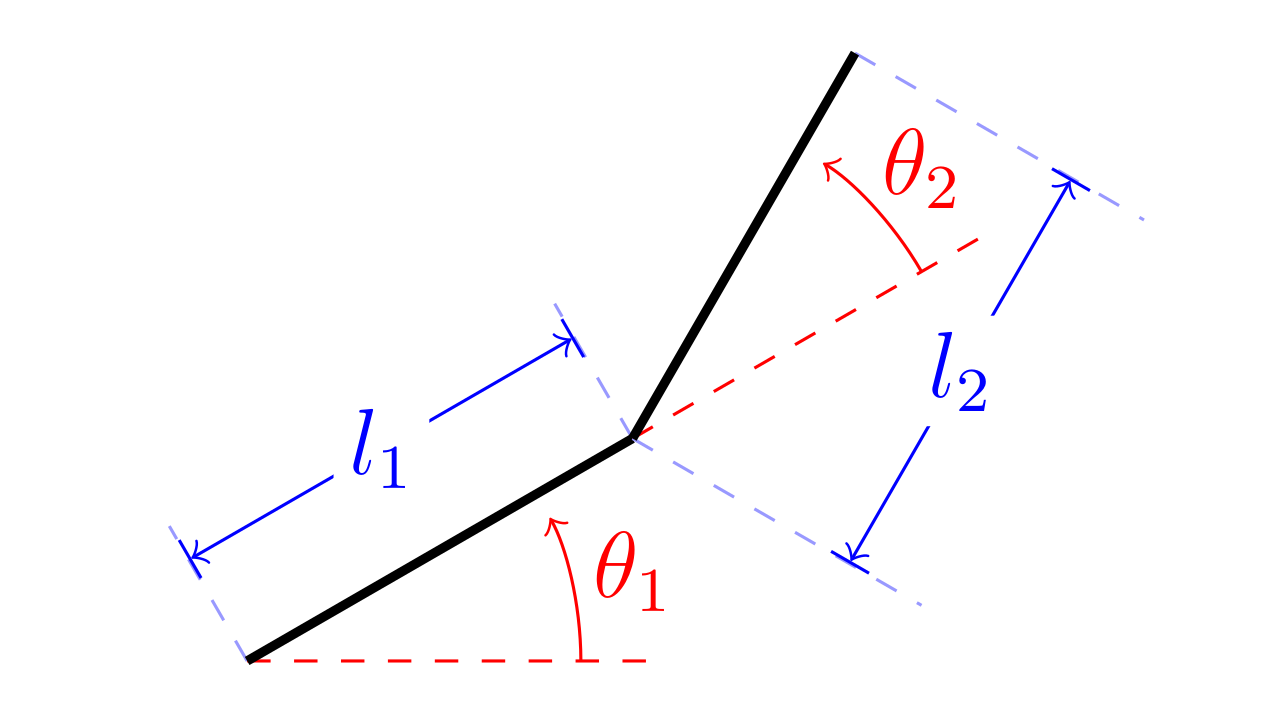
\includegraphics[width=8cm]{figures/2R.png}
    \caption{$q$ or $\theta$ assignment for a 2R agent.}
    \label{fig:2R}
\end{figure}

\subsection{Tree of NR chains agent}
Multiple NR chain agents can be joined end-to-end to form a tree.
The ends where joining occurs cannot be used as a pivot.
At any point of time exactly one pivot.
For a (parent, child) NR chain pair, we assume that the point of joining is controlled by the parent agent.
The child agent uses the point of joining as it's pivot.
Figure \ref{fig:2} shows examples of such agents.
Such a $2 \times 2R$ agent is used to model two arms or two legs.
The difference between a $4R$ agent and a $2 \times 2R$ agent is that the latter can be controlled hierarchically.
Thus multiple elements can be composed without much agent specific math.
The methods discussed in this work are implemented for $2 \times 2R$ agent modeling two arms, but are mostly applicable for any Tree of NR chains agent.
\begin{figure}[h!]
    \centering
    \begin{tikzpicture}
    \draw[red] (-1,0) -- (0,1); \draw[red] (0,1) -- (1,0);
    \draw[green] (1,0) -- (2,1); \draw[green] (2,1) -- (3,0);

    \draw[red] (4,0) -- (5,1); \draw[red] (5,1) -- (6,0);
    \draw[green] (6,0) -- (7,1); \draw[green] (7,1) -- (8,0);
    \draw[blue] (8,0) -- (9,1); \draw[blue] (9,1) -- (10,0);

    \draw[red] (11,0) -- (12,1); \draw[red] (12,1) -- (13,0);
    \draw[green] (13,0) -- (14,1); \draw[green] (14,1) -- (15,0);
    \draw[blue] (13,0) -- (14,-1); \draw[blue] (14,-1) -- (13,-2);
    \end{tikzpicture}
    \caption{$2 \times 2R$, $3 \times 2R$ agents.}
    \label{fig:2}
\end{figure}

\subsection{Environment}
A 2D wall with holds is the environment.
A free end can reach a hold and can use it as a pivot.
In that case the existing pivot becomes a free end to maintain the invariant of exactly one pivot.
An example is shown is figure \ref{fig:3}.
\begin{figure}[h!]
    \centering
    \begin{tikzpicture}
    \draw (0,0) rectangle (10,10);
    \filldraw [red] (1,1) circle (5pt);
    \filldraw [black] (1,2) circle (2pt);
    \filldraw [black] (2,2) circle (2pt);
    \filldraw [black] (2.5,1) circle (2pt);
    \filldraw [black] (3.5,4) circle (2pt);
    \filldraw [black] (4,3) circle (2pt);
    \filldraw [black] (5,3) circle (2pt);
    \filldraw [black] (6,4) circle (2pt);
    \filldraw [black] (6,4.5) circle (2pt);
    \filldraw [black] (8,6) circle (2pt);
    \filldraw [black] (7,6) circle (2pt);
    \filldraw [black] (6,8) circle (2pt);
    \filldraw [black] (5,9) circle (2pt);
    \filldraw [black] (5,8) circle (2pt);
    \filldraw [black] (4,8.5) circle (2pt);
    \filldraw [black] (3,8) circle (2pt);
    \filldraw [black] (2,9) circle (2pt);
    \filldraw [green] (2,9) circle (5pt);
    \end{tikzpicture}
    \caption{Wall environment. Dots are holds. Red dot is start hold. Green dot is finish hold.}
    \label{fig:3}
\end{figure}

\subsection{Motivation and broader use}
Firstly it is quite fun to watch robots climb walls.
But also by solving this problem one can find solutions for new and potentially dangerous bouldering problems.
If implemented in real robots, they can be used to climb difficult and challenging terrain for reconnaissance or rescue missions.
In terms of animation, most games use fixed climb cycles.
This method can be used to improve climbing character animation.

\section{related work}
In general the problem of motion planning for wall-climbing is not as explored as other tasks like running, jumping, dribbling and even swimming.
\cite{bull1995adaptive} propose wall climbing robot gait control using genetic algorithms and Q-learning.
\cite{Grieco1998ASC} and \cite{351225} demonstrate real life wall-climbing robots. The dynamics of their robot are similar to agents considered in this work.
\cite{kalisiak2001grasp} is one of the first papers to work on animating 2D parkour agents involving swinging, climbing and crawling. They propose a kinematic motion planning algorithm based on stochastic search procedures guided by geometric constraints. This work also uses random sampling to solve for globally optimal inverse kinematics.
\cite{10.1145/3072959.3073707} addresses the problem of offline path and movement planning for wall climbing humanoid agents.
\cite{2017-TOG-deepLoco} uses the idea of hierarchical controller generation for the tasks of walking, running, jogging, dribbling etc. This idea of hierarchical control is used in this work. A neural network is used to plan goals for a lower level inverse kinematics solver.
\subsection{Baseline}
Baseline is chosen as my previous work on this problem.
The source code, demo and report can be found at \url{https://github.com/buggedbit/stick-solo}.
The baseline considers similar NR chain agents but it
\begin{enumerate}[nolistsep]
    \item Has no constraints on $q_i$ and $\Delta q_i$.
    \item Has no center of mass considerations.
    \item Has no multi-limb coordination.
    \item Mainly uses gradient descent on loss function.
    $
            \Delta q \equiv -\frac{\delta (goal - end)^2}{\delta q}
    $
\end{enumerate}
One of the main problems of the baseline, more specifically the gradient descent, is the possibility of local minima.
Combined with no constraints on $q_i$ and $\Delta q_i$, modeling limbs using these agents this produces weird poses and transformations between poses.
These issues are addressed in this work.
\subsection{Oracle}
There are two components of evaluation in this problem.
\begin{enumerate}[nolistsep]
    \item Reaching the goal.
    \item Moving in a human-like way.
\end{enumerate}
While the first one can be evaluated automatically, the latter one is best evaluated using user-studies.
\subsection{Contribution}
The main contribution of this work over baseline is to
\begin{enumerate}[nolistsep]
    \item Add constraints on $q_i$ and $\Delta q_i$.
    \item Add center of mass terms to the loss function to model natural human motion.
    \item Develop arbitrarily close globally optimal solves for NR chain agents.
    \item Formulating and implementing the control of $2 \times NR$ as an RL problem.
\end{enumerate}

\section{approach}
In this section the approach is incrementally presented.

\subsection{Constraints on $q_i$ and $\Delta q_i$}
For each join of the agent two constraints; one on its value and one on its rate of change is implemented.
Any rate of change of magnitude more than certain threshold is clamped.
Similarly if a change in joint angle makes its magnitude more than a certain threshold then the angle is clamped.

\subsection{Gradient descent on center of mass}
Baseline uses gradient descent on the following loss function.
\[
    L \equiv (goal - end)^2
\]
So an update on $q_i$s would be
\[
    \Delta q \equiv -\frac{\delta L}{\delta q}
\]
But this does not explicitly model any nature of motion, and therefore there are no preferred joint angles.
To make the motion more natural, the most basic thing to simulate is gravity.
Since simulating forces and torques on each link and interaction forces b/w all pairs of touching links would be cumbersome, we simulate its effect on the center of mass of the whole agent.
We try to bring the center of mass of the whole body down and towards the midpoint of current pivot and current goal.
Therefore the loss function becomes
\[
    L \equiv \alpha * (goal - end)^2 + \beta * (com_x - (goal_x - pivot_x) / 2)^2 + \gamma com_y
\]
where $\alpha, \beta, \gamma$ are tunable constants.
Higher values of $\alpha$ models stronger agents, while lower values model weaker agents.
Now the update becomes
\[
    \Delta q
    \equiv -\frac{\delta L}{\delta q}
    \equiv
    - \alpha \frac{\delta (goal - end)^2 }{\delta q}
    - \beta \frac{\delta (com_x - (goal_x - pivot_x) / 2)^2 }{\delta q}
    - \gamma \frac{\delta com_y}{\delta q}
\]
The first term is already calculated in the baseline.
The other terms can be easily calculated once
\[
    \frac{\delta com_x }{\delta q},
    \frac{\delta com_y }{\delta q}
\]
are known.
\\\\
Consider
\[
    \frac{\delta com_x }{\delta q}
\]
Assuming same mass for all links and given x-coordinates of vertices of NR chain
\[
    x_0, x_1, ... x_n
\]
The x-coordinate center of mass of each link will be at its center
\[
    c_i \equiv (x_i + x_{i + 1}) / 2; i = 0, 1, ... n - 1
\]
Therefore x-coordinate of center of mass of entire agent is
\[
    com_x \equiv x_0/2 + x_1 + x_2 + ... + x_{n-1} + x_n / 2
\]
But from the dynamics of NR chain we know that
\[
    x_i \equiv \sum_{i = 1}^{n} l_i cos(\sum_{j = 1}^{i} q_j)
\]
\[
    y_i \equiv \sum_{i = 1}^{n} l_i sin(\sum_{j = 1}^{i} q_j)
\]
Thus we have formulated $com_x$ in terms of $q_i$s, which makes calculating
\[
    \frac{\delta com_x }{\delta q}
\]
feasible.
The calculation of
\[
    \frac{\delta com_y }{\delta q}
\]
follows the same arguments.
The effect of this term is illustrated in figure \ref{fig:com_effect}.
\begin{figure}[h]
    \centering
    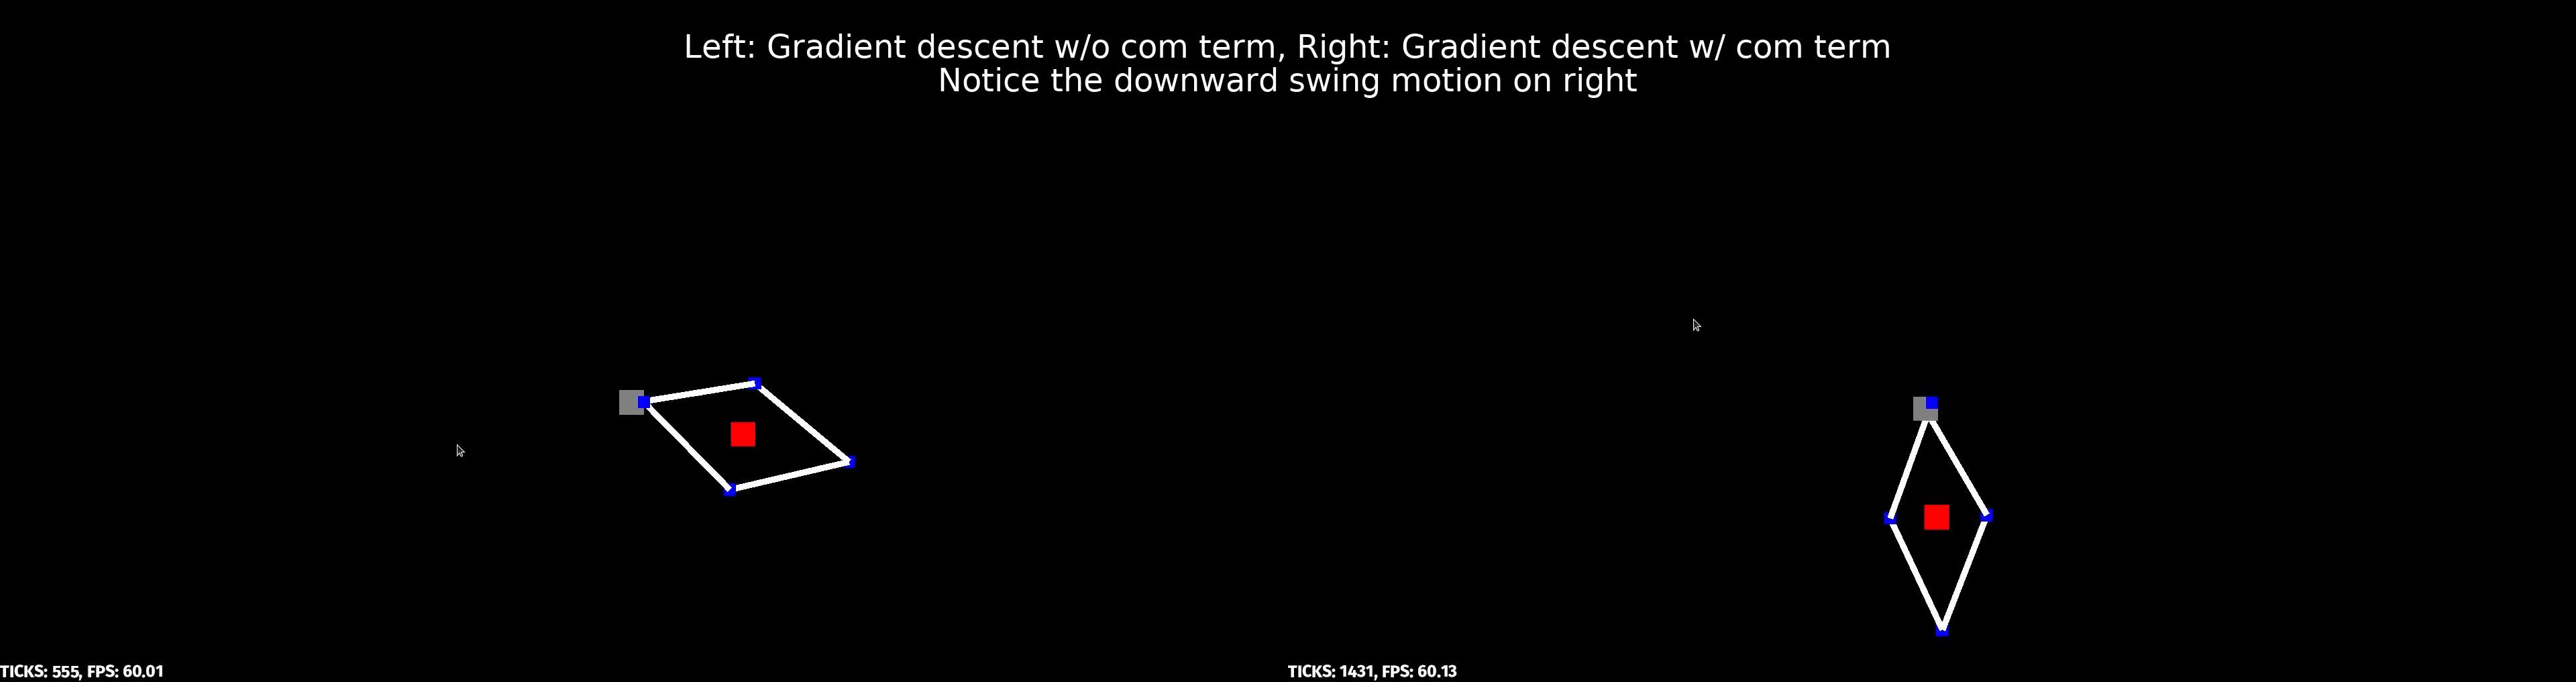
\includegraphics[width=16cm]{figures/com_effect.jpg}
    \caption{Left agent has no com control, therefore stays in a tilted position. Right agent has com control, therefore swings downward.}
    \label{fig:com_effect}
\end{figure}
\paragraph{Notes}
In practice we found it better to have more discounted com control for links farther from pivot since it is natural for them to be more responsible about reaching the goal rather than maintaining com position.
Also observe that the goal for x-coordinate for center of mass can be changed with very little change in math.
For both terms the gradient becomes zero at both local minima and local maxima.
Ideally the local maxima case should be handled explicitly.
But since it is an unstable equilibrium and there is almost always a perturbation from some other control (like from the first term).
Therefore it is very rare for the agent to be stuck at local maxima and hence handling it explicitly is not needed in practice.
\paragraph{Time complexity}
Computing these terms has $O(n^3)$ time complexity when done in a brute force way.
But due to the repeated summations it is actually possible prune some computations by maintaining total sums and subtracting from them.
This approach has $O(n^2)$ time complexity, which is the one implemented in the code.
But since for the purposes of this work we are considering single NR agents with small N, it does not make much difference.
However if work-like agent (NR chain with large N) or large crowds of climbing agents are simulated then this can make a significant difference.

\subsection{Globally optimal inverse kinematics solves}
Gradient descent with constraints can cause agents getting stuck at local minima poses.
This is illustrated in figure \ref{fig:local_minima}.
Even though this can be mitigated a bit with parameter tuning it is still an intrinsic and major problem.
To solve this we need a globally optimal solve for inverse kinematics under constraints.
But there is no generalized inverse kinematics solve for NR chain agents for $N > 2$ yet.
To solve this we can soften the requirement to solve for arbitrarily close globally optimal solves.

\begin{figure}[!htb]
\minipage{0.32\textwidth}
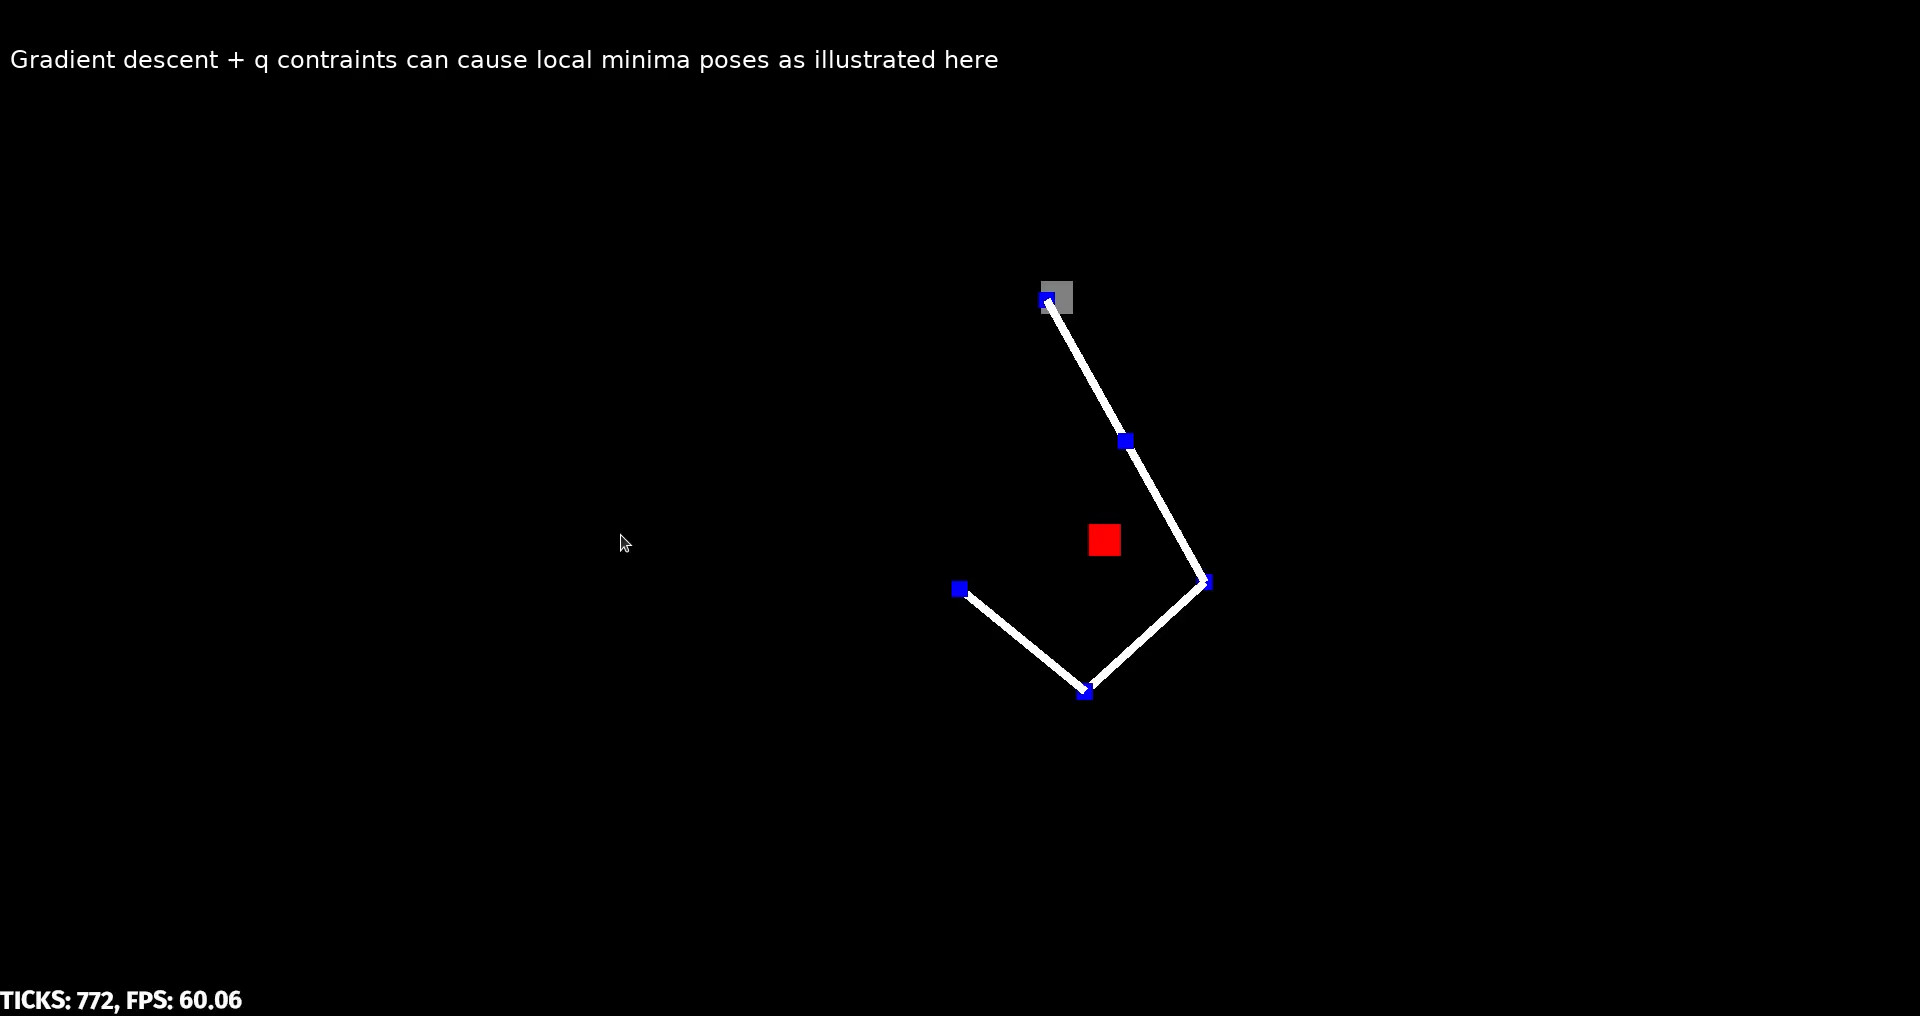
\includegraphics[width=\linewidth]{figures/1.a.jpg}
\endminipage\hfill
\minipage{0.32\textwidth}
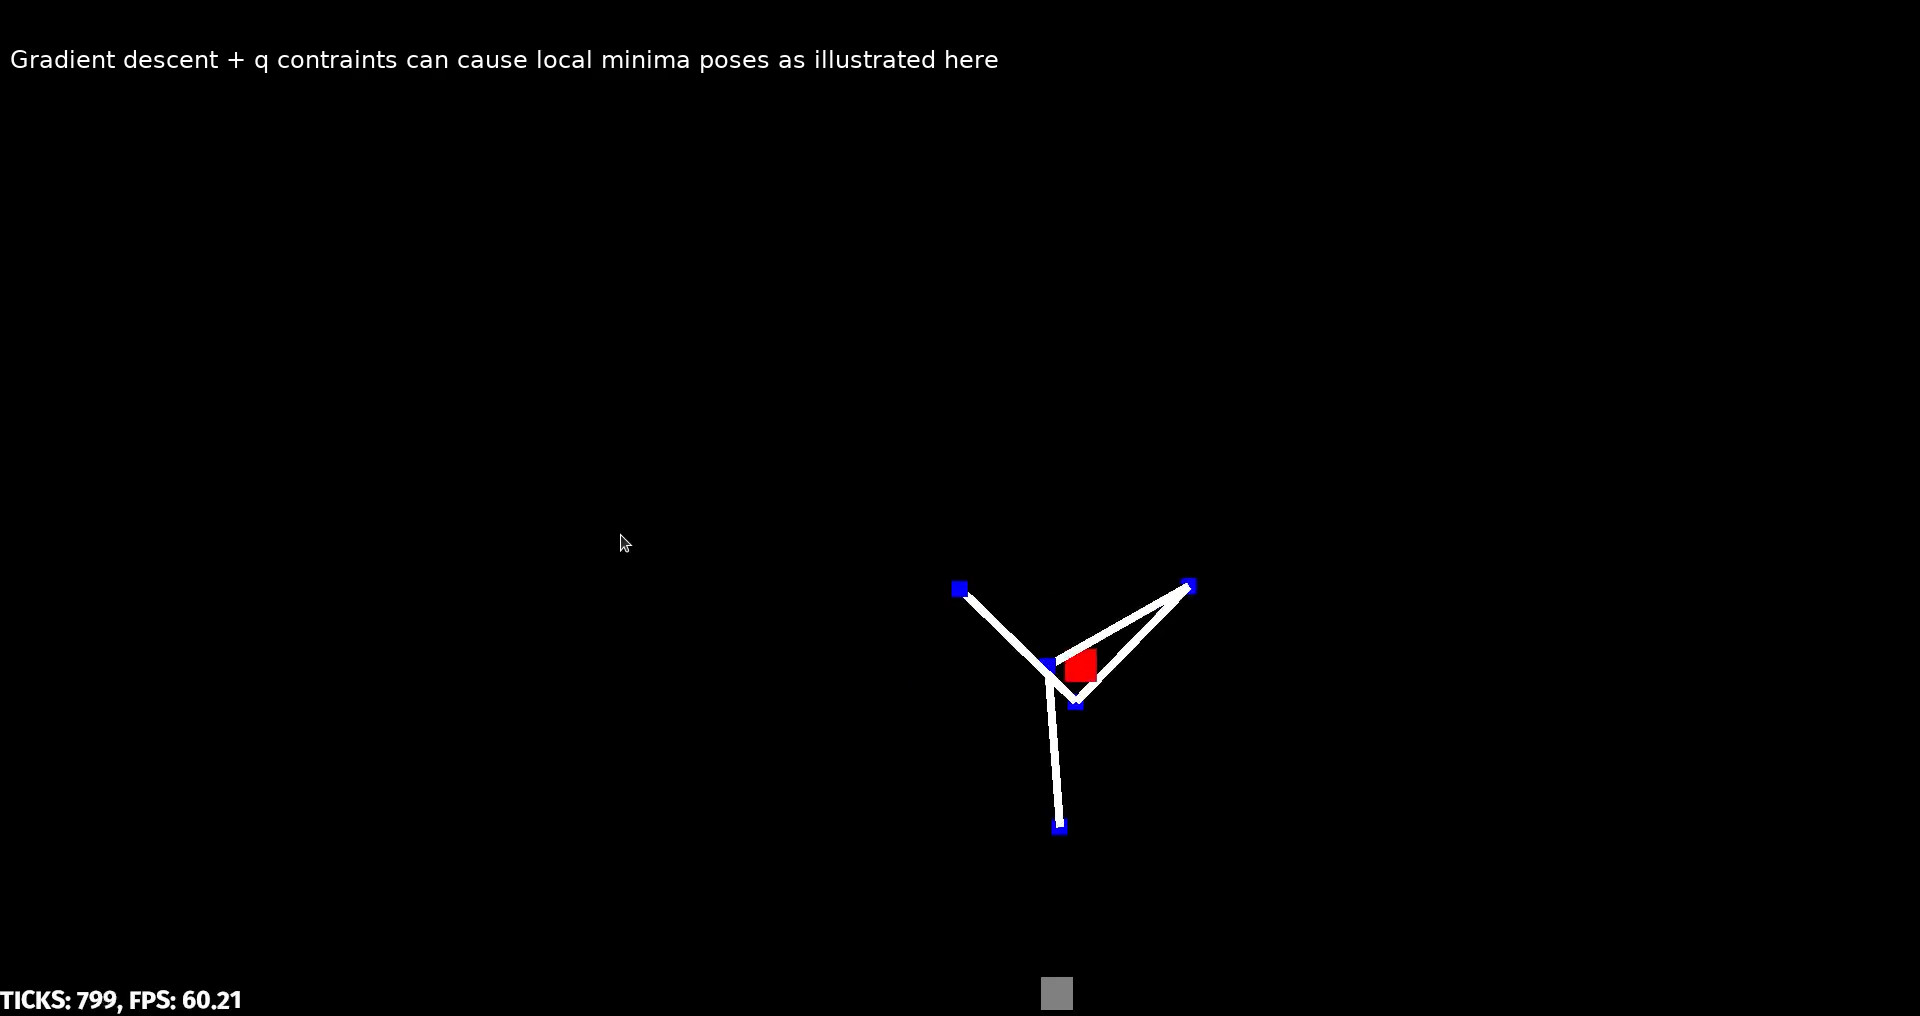
\includegraphics[width=\linewidth]{figures/1.b.jpg}
\endminipage\hfill
\minipage{0.32\textwidth}%
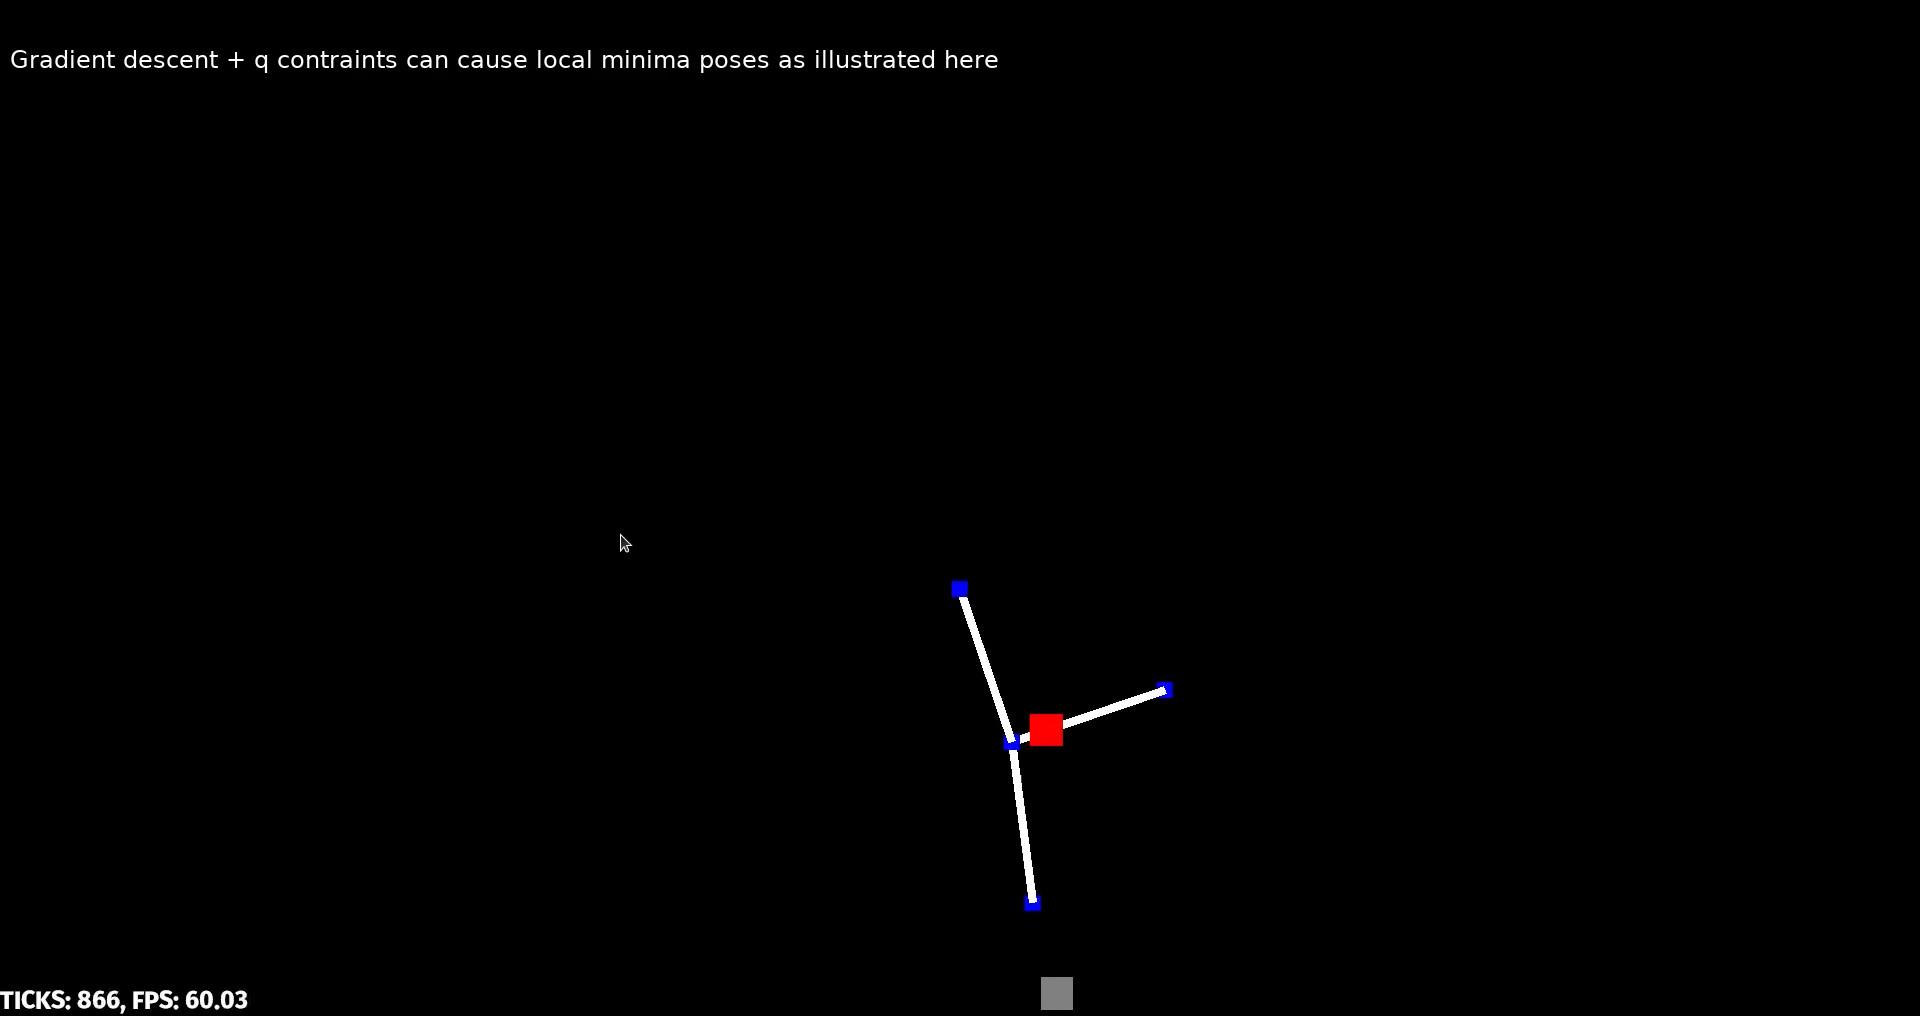
\includegraphics[width=\linewidth]{figures/1.c.jpg}
\endminipage
\\
\minipage{0.32\textwidth}
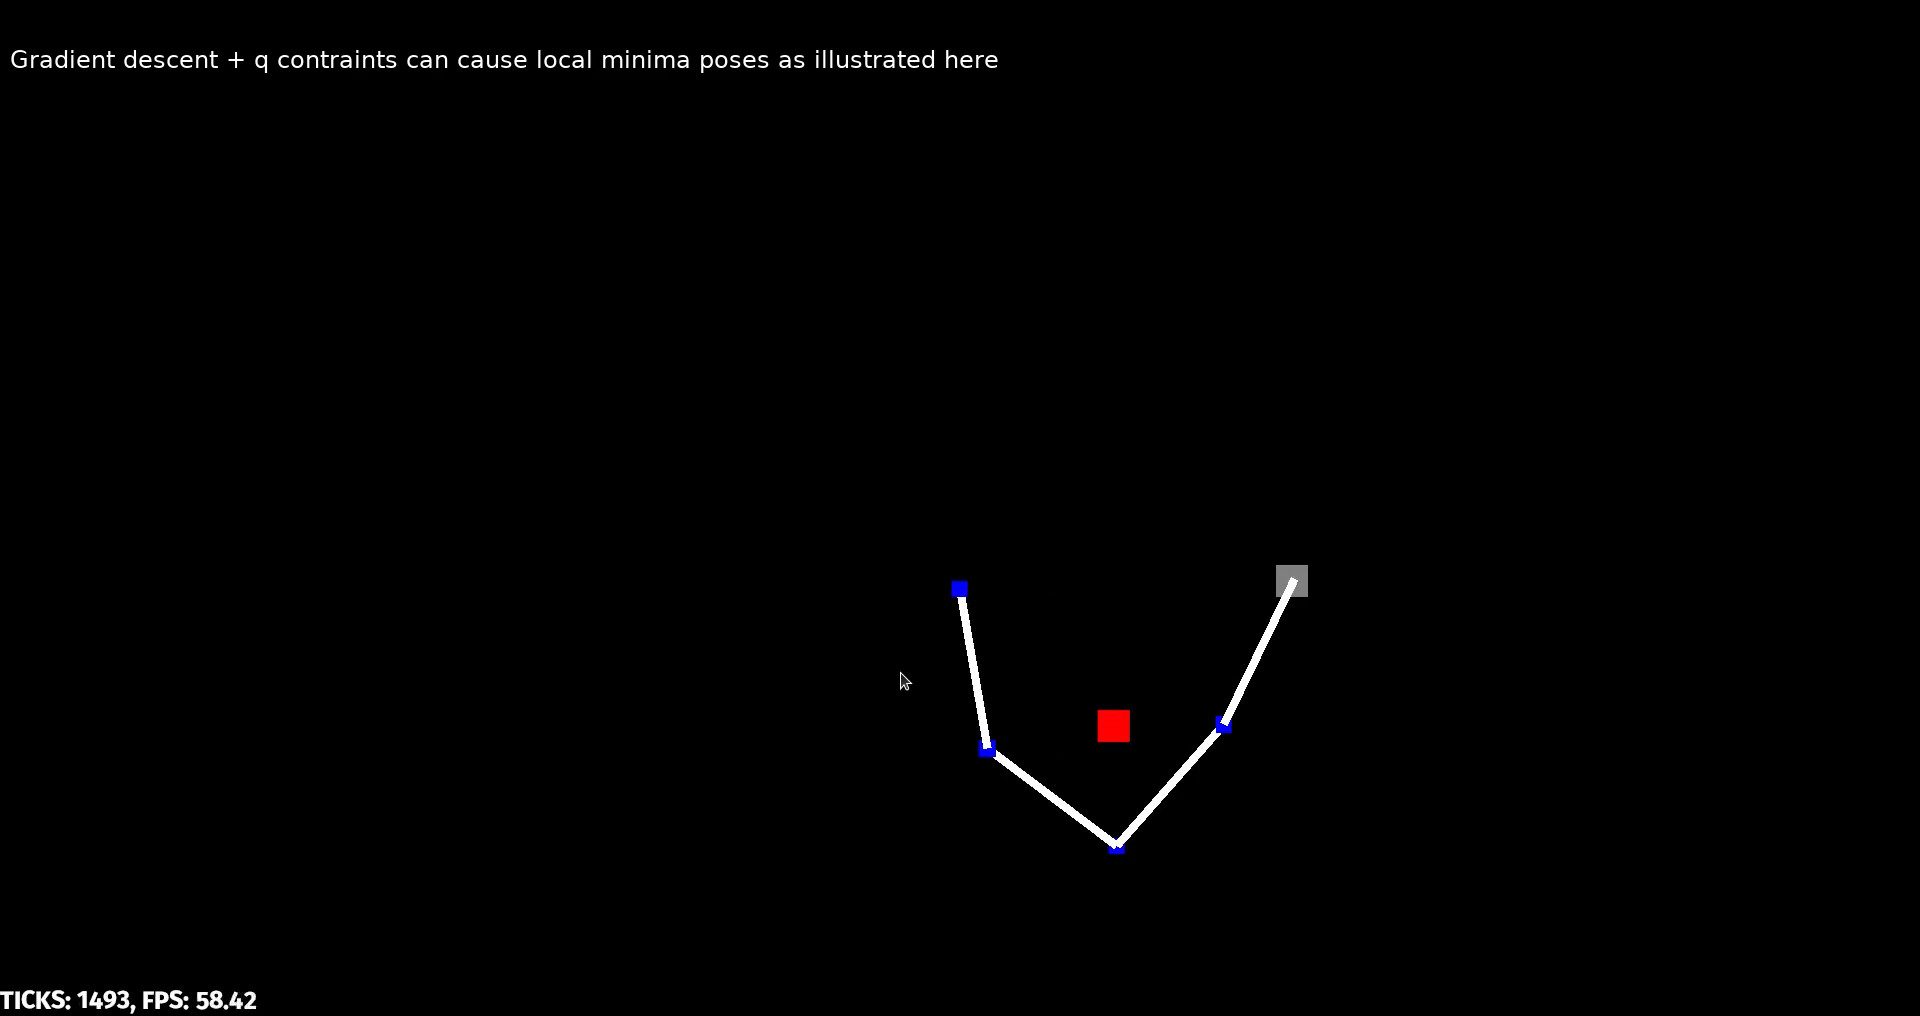
\includegraphics[width=\linewidth]{figures/2.a.jpg}
\endminipage\hfill
\minipage{0.32\textwidth}
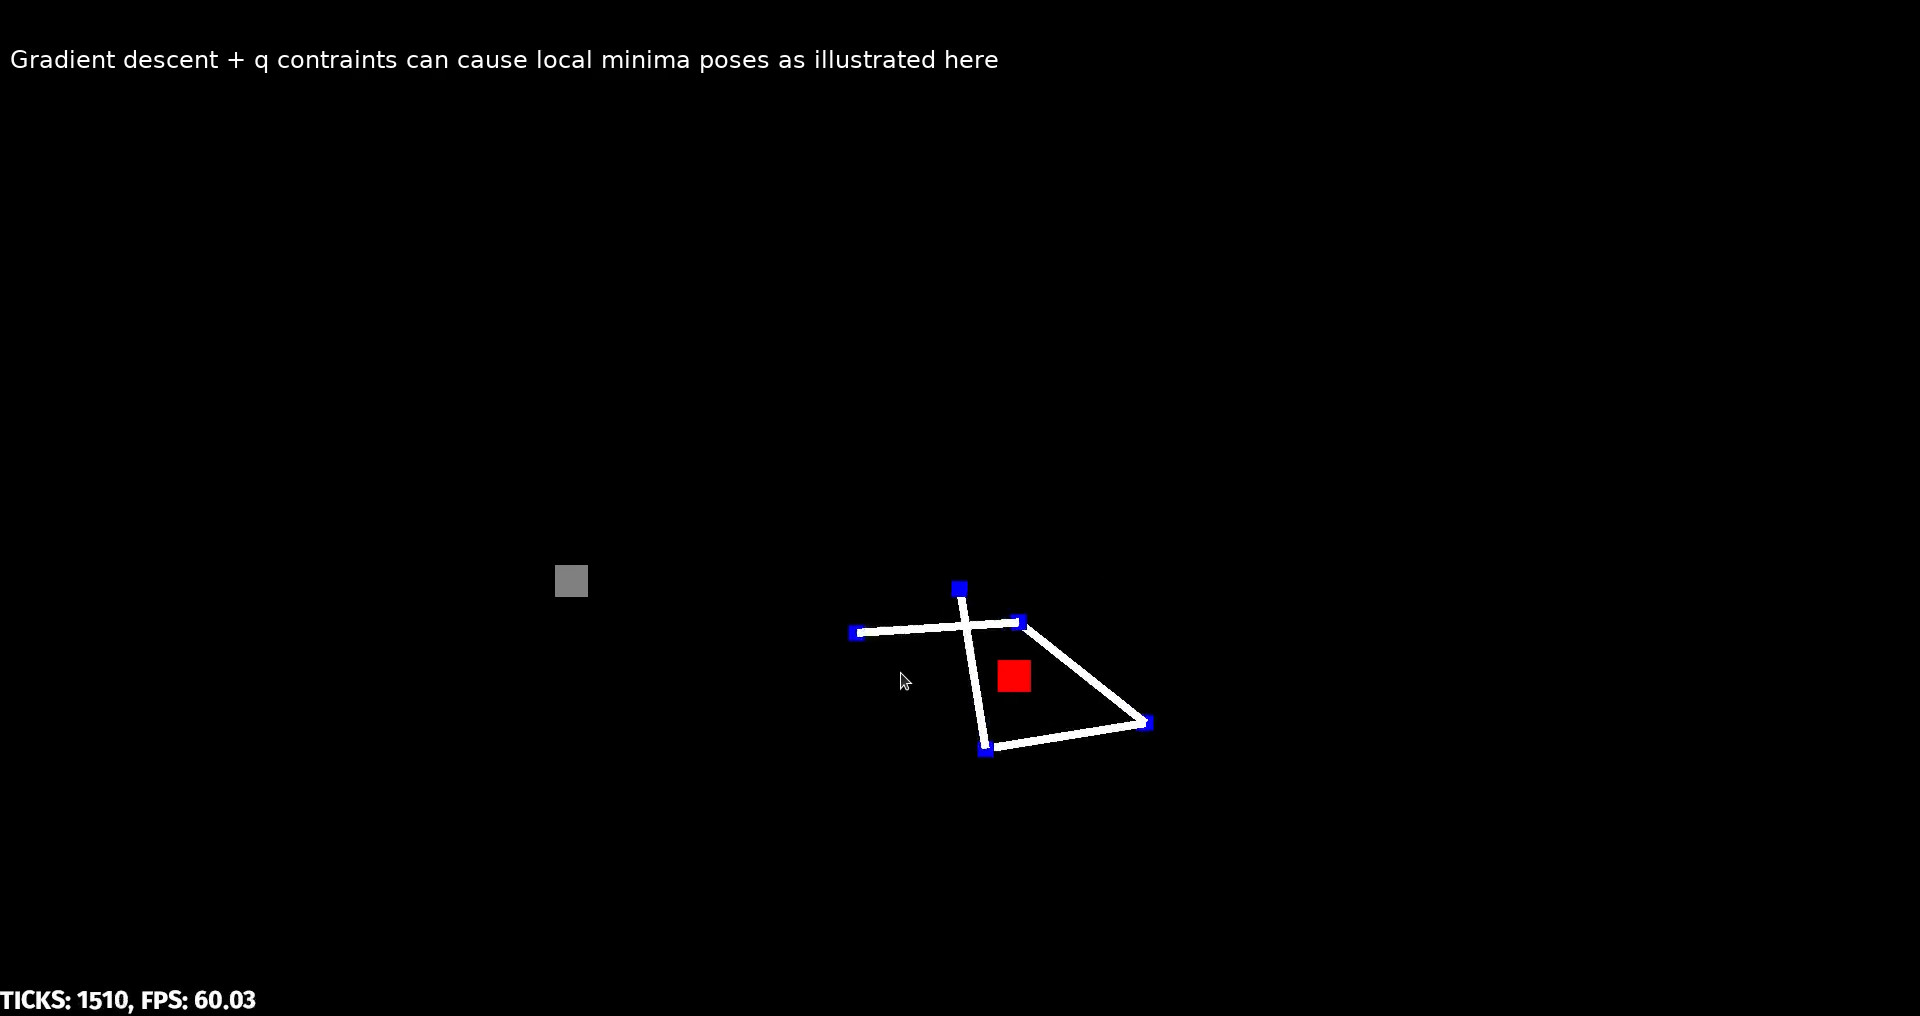
\includegraphics[width=\linewidth]{figures/2.b.jpg}
\endminipage\hfill
\minipage{0.32\textwidth}%
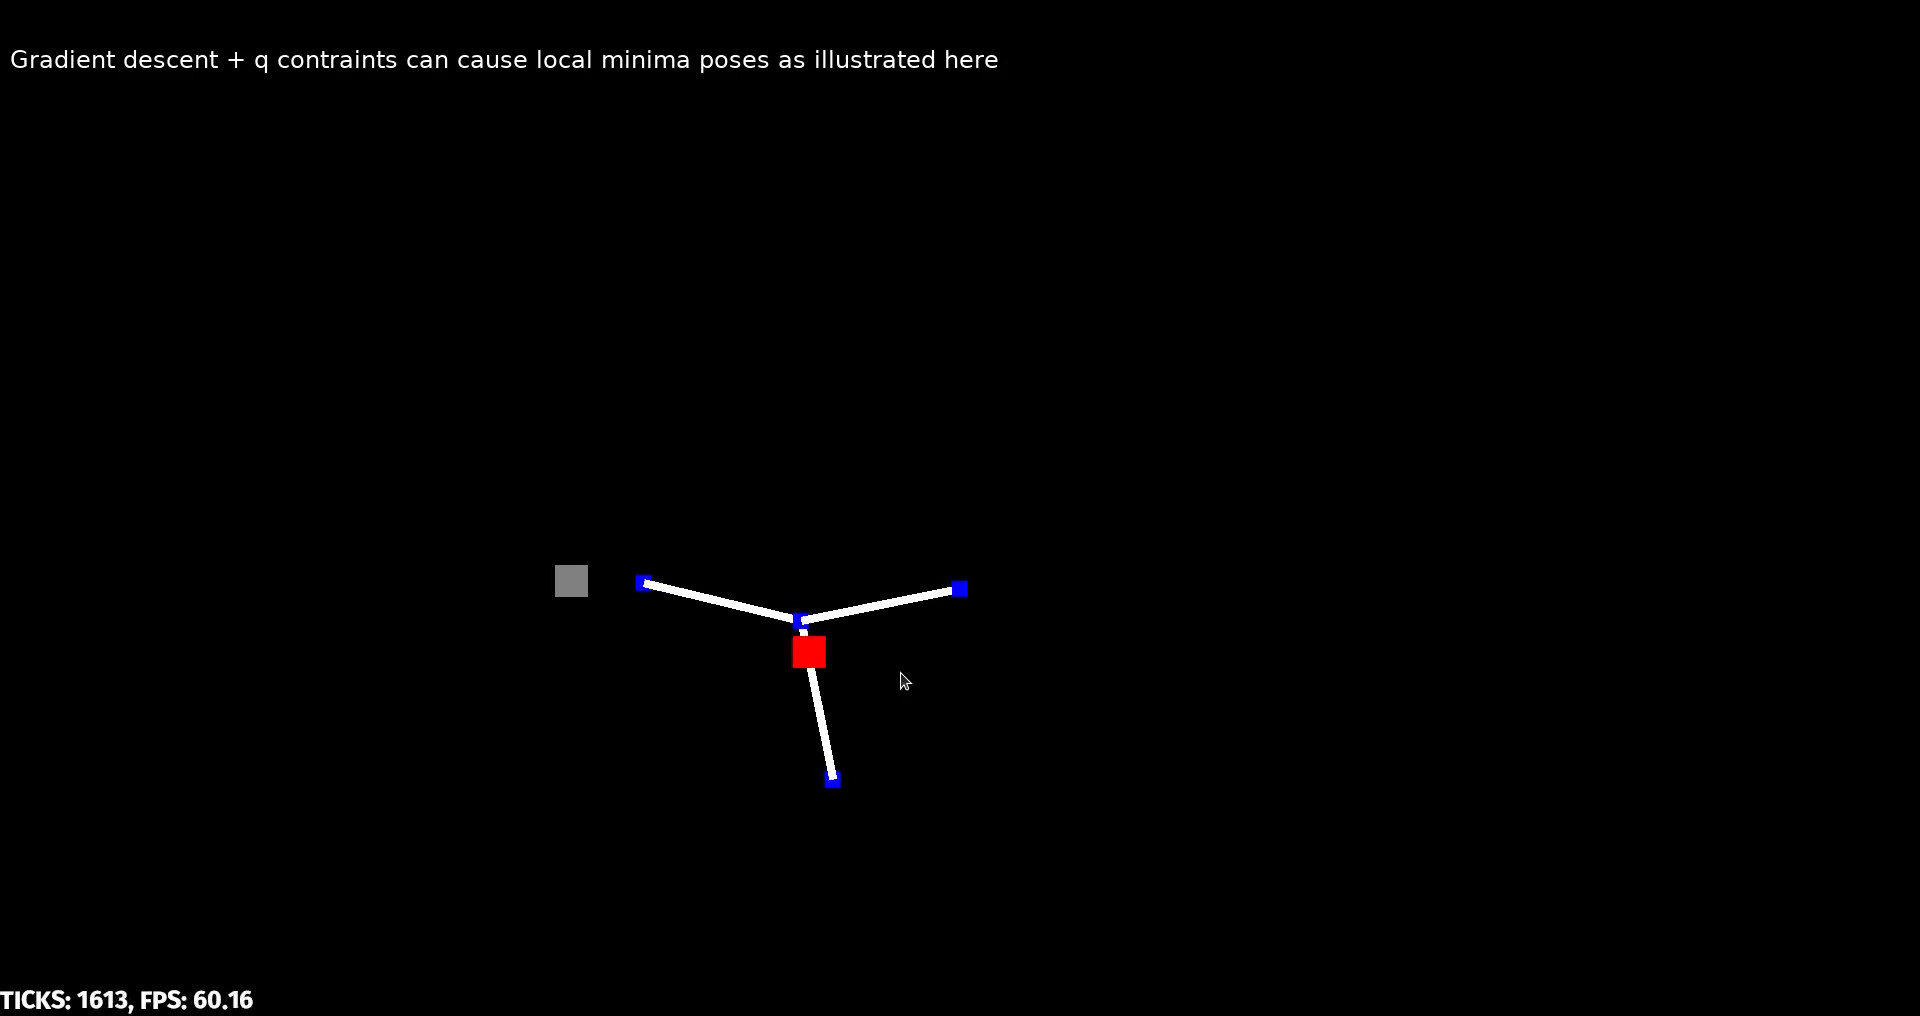
\includegraphics[width=\linewidth]{figures/2.c.jpg}
\endminipage
\caption{Top 3 one motion, Bottom 3 one motion. Agent crosses arms to get stuck in a local minima pose.}
\label{fig:local_minima}
\end{figure}

\subsection{No prior random sample solve}
From the spirit of RANSAC, this is a simple method based on randomization.
Given a goal, randomly sample $q$s (in their ranges) and keep the track of $q^*$ which achieves closest approach.
This can be stopped after a fixed number of samples or if closest approach is less than a threshold.
This at limit should not be stuck at local minima and therefore is a arbitrarily near optimal solve.
Given $q^*$ just interpolate from current q to $q^*$ to reach the goal.
Since the distance calculation part is independent for each randomly sampled $q$, that part of the algorithm is parallelizeable.
Since the actual function which ranks sampled $q$s can be arbitrary, we can actually use this to optimize more compound loss functions.
For example in the implementation
\[
    L \equiv \alpha * (goal - end)^2 + \beta * (com_x - (goal_x - pivot_x) / 2)^2 + \gamma com_y
\]
is globally optimized.

\subsection{Current state random sample solve}
From the spirit of genetic algorithms, this is a simple method based on randomization, similar to no prior random sample solve.
Instead of sampling $q$s randomly in whole range, we sample in small region around current $q$, set the best $q^*$ as the new $q$ and repeat.
This method is more prone to local minima than previous method but given enough big sampling vicinity local minima can be avoided.
Therefore this is asymptotically equivalent to no prior random sample solve.
On the other hand this method is faster than the former, especially when number of dimensions of $q$ space is large, since it only samples in a small vicinity around current $q$. Therefore this method scales better with $q$ dimension and/or number of agents.

\subsection{Integration with gradient descent}
Both of the above solves are implemented and presented in the demo.
But even with the globally optimal solve, most of the times, we do not exactly reach global minima but shall be in a close but unknown vicinity of it, depending on number of samples and dimension of $q$ space.
Since for continuing on a wall we need to actually get to a specified distance from the goal, we cannot just rely on these globally optimal solves.
Therefore we first use globally optimal control to get within a close vicinity of global minima and then switch to gradient descent for ensuring reaching the goal.
In practice we found that
\[
    \alpha * c_{global} + \beta * c_{gradient\_descent}; \alpha = \frac{1}{(1 + ticks)^{0.5}}, \beta = 1 - \alpha
\]
works well for our demos; where $ticks$ is the number of ticks completed from initial pose where globally optimal solve $q\*$ was calculated.
Using these methods the agents were able to avoid getting stuck in local minima poses.

\subsection{Switching pivot}
When the goal is reached by a free end, then the agent has to switch pivot.
Switching pivot is essentially changing the pivot position, order of lengths of links, $q_i$s and $q_{i}clamps$.
When pivot is switched
\begin{enumerate}[nolistsep]
    \item Pivot position is the previous end position.
    \item Order of lengths of links are reversed.
    \item From the dynamics $q_{new} = [\sum_{i=1}^{n} q_i - \pi, -q_{n-1}, ..., -q_{1}]$.
    \item From the dynamics $q_{new}clamps = [...(-q_imax, -q_imin)]; i = 1, 2, ..., n$.
\end{enumerate}
We can see from points 3 and 4 that the first $q$ is in general not bounded. Therefore the $q_1clamps$ have to be $(-\infty, \infty)$.
This means that we cannot enforce constraints on first joint angle if we want to switch pivot generally.
This becomes a problem when one goal is high up the pivot and the next goal is low below the pivot, in which case agent tends to make unnatural cartwheeling motion.
This is illustrated in figure \ref{fig:cartwheel}.
\begin{figure}[!htb]
\minipage{0.32\textwidth}
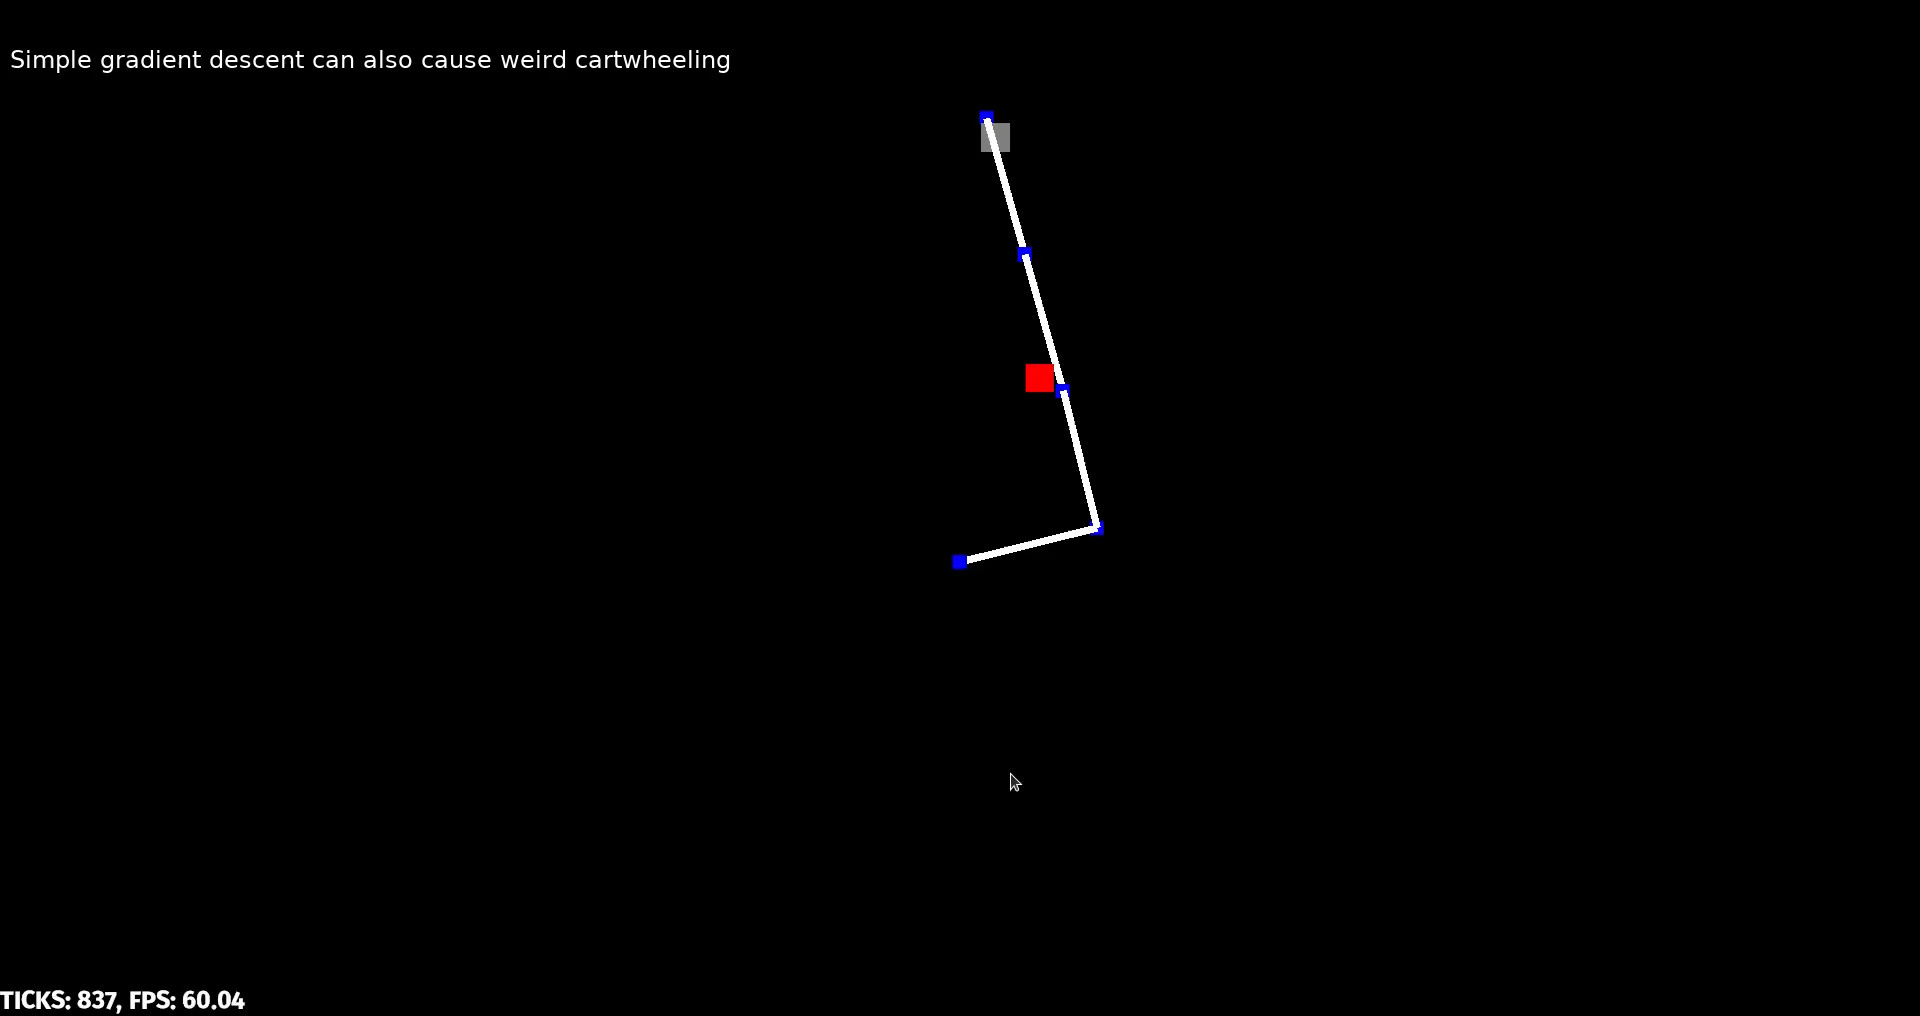
\includegraphics[width=\linewidth]{figures/cw1.jpg}
\endminipage\hfill
\minipage{0.32\textwidth}
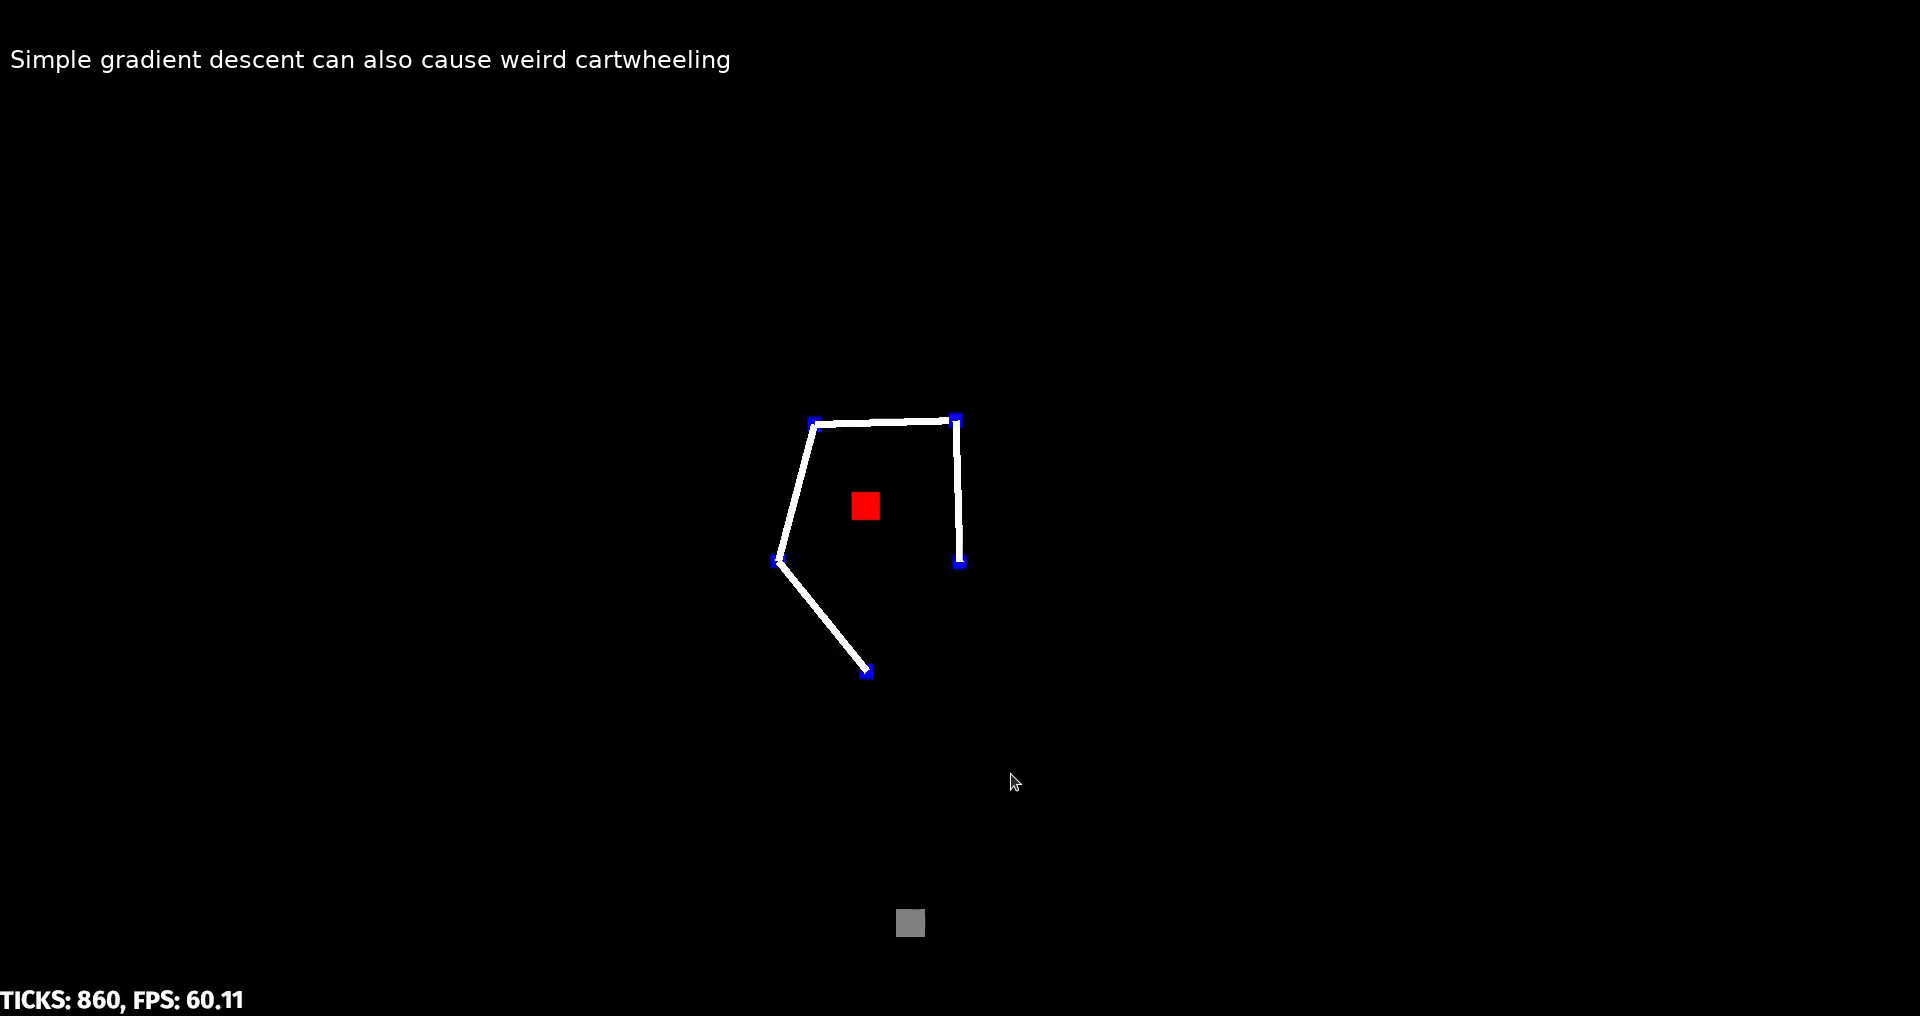
\includegraphics[width=\linewidth]{figures/cw2.jpg}
\endminipage\hfill
\minipage{0.32\textwidth}%
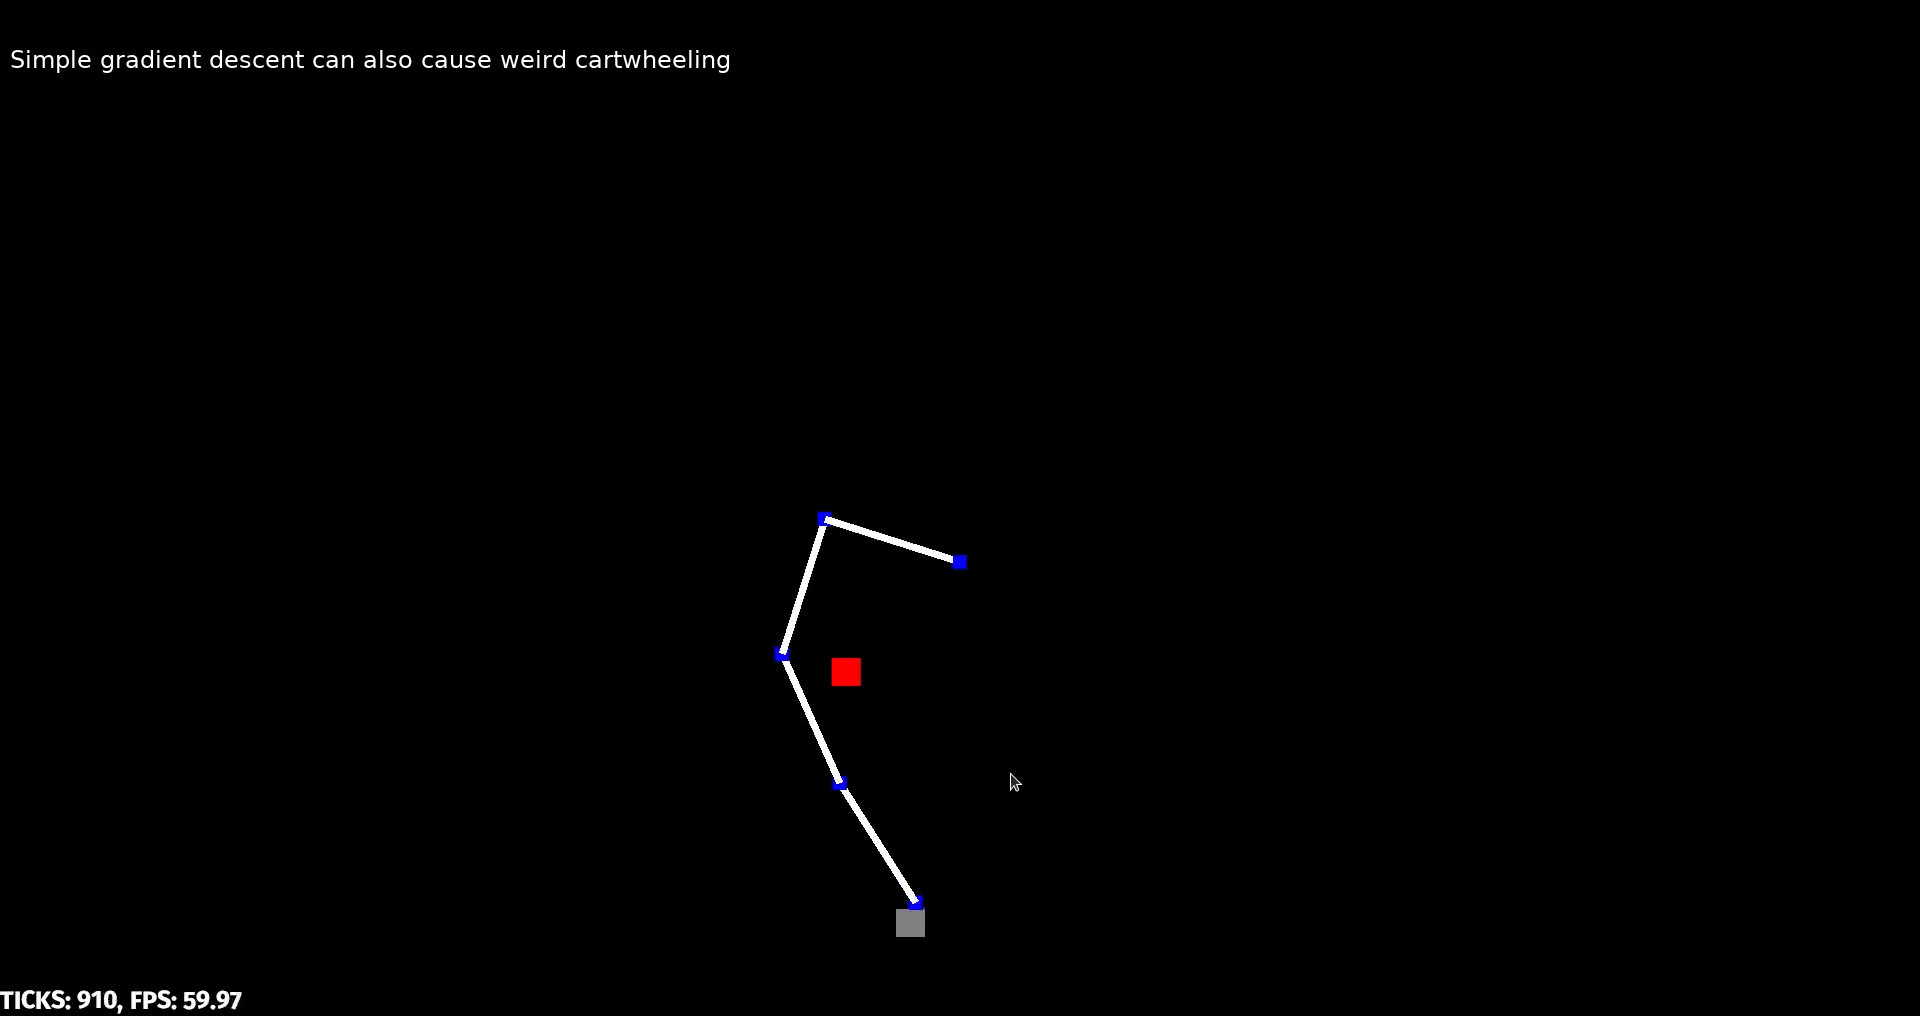
\includegraphics[width=\linewidth]{figures/cw3.jpg}
\endminipage
\caption{Left hand pivoting agent makes a cartwheel in attempt to reach the goal, because constraints cannot be enforced on $q_1$.}
\label{fig:cartwheel}
\end{figure}
This can be solved by only sampling certain range of $q_1$ values while performing globally optimal solves.

\subsection{Matching hands}
This alternating hand + switching pivot method does not always work as illustrated in figure \ref{fig:sf}.
This can be resolved by matching hands.
\begin{enumerate}[nolistsep]
    \item If agent is reaching with left hand but goal on on right of pivot, set goal as pivot.
    \item If agent is reaching with right hand but goal on on left of pivot, set goal as pivot.
\end{enumerate}
This is illustrated in figure \ref{fig:m}
\begin{figure}[!htb]
\minipage{0.32\textwidth}
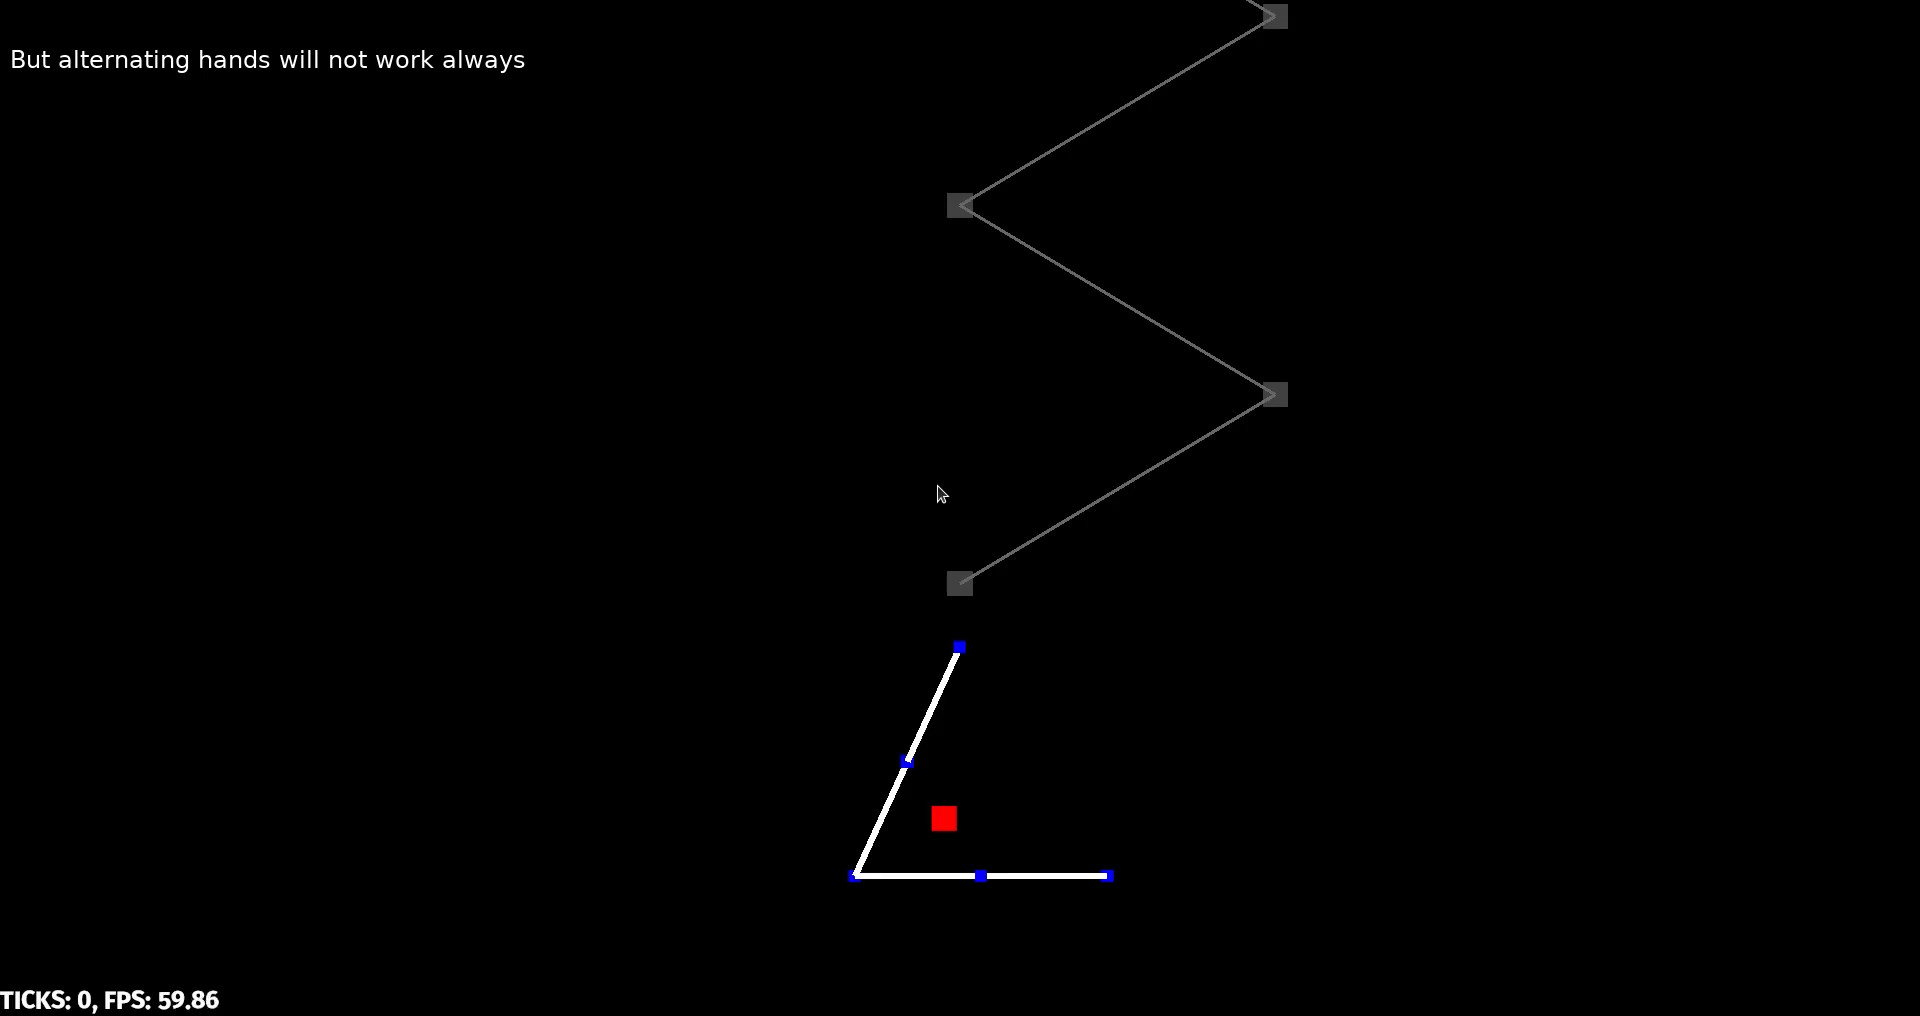
\includegraphics[width=\linewidth]{figures/sf1.jpg}
\endminipage\hfill
\minipage{0.32\textwidth}
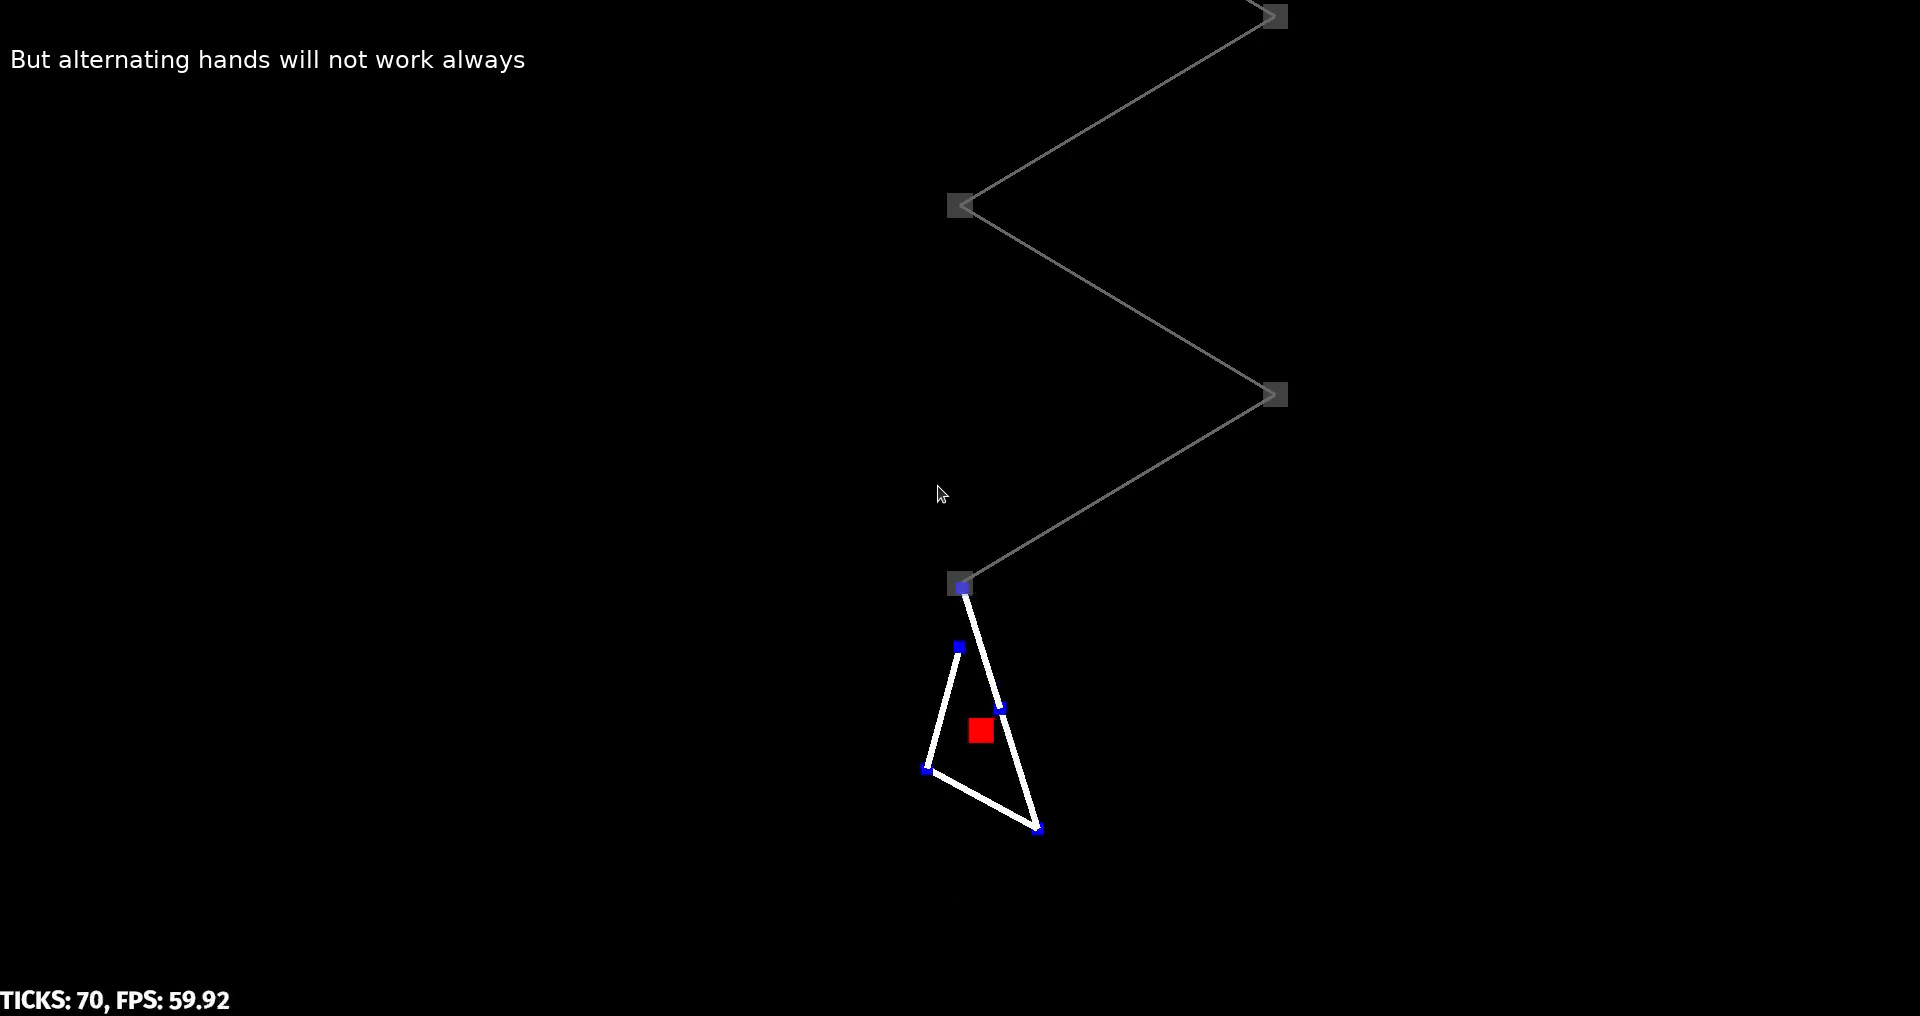
\includegraphics[width=\linewidth]{figures/sf2.jpg}
\endminipage\hfill
\minipage{0.32\textwidth}%
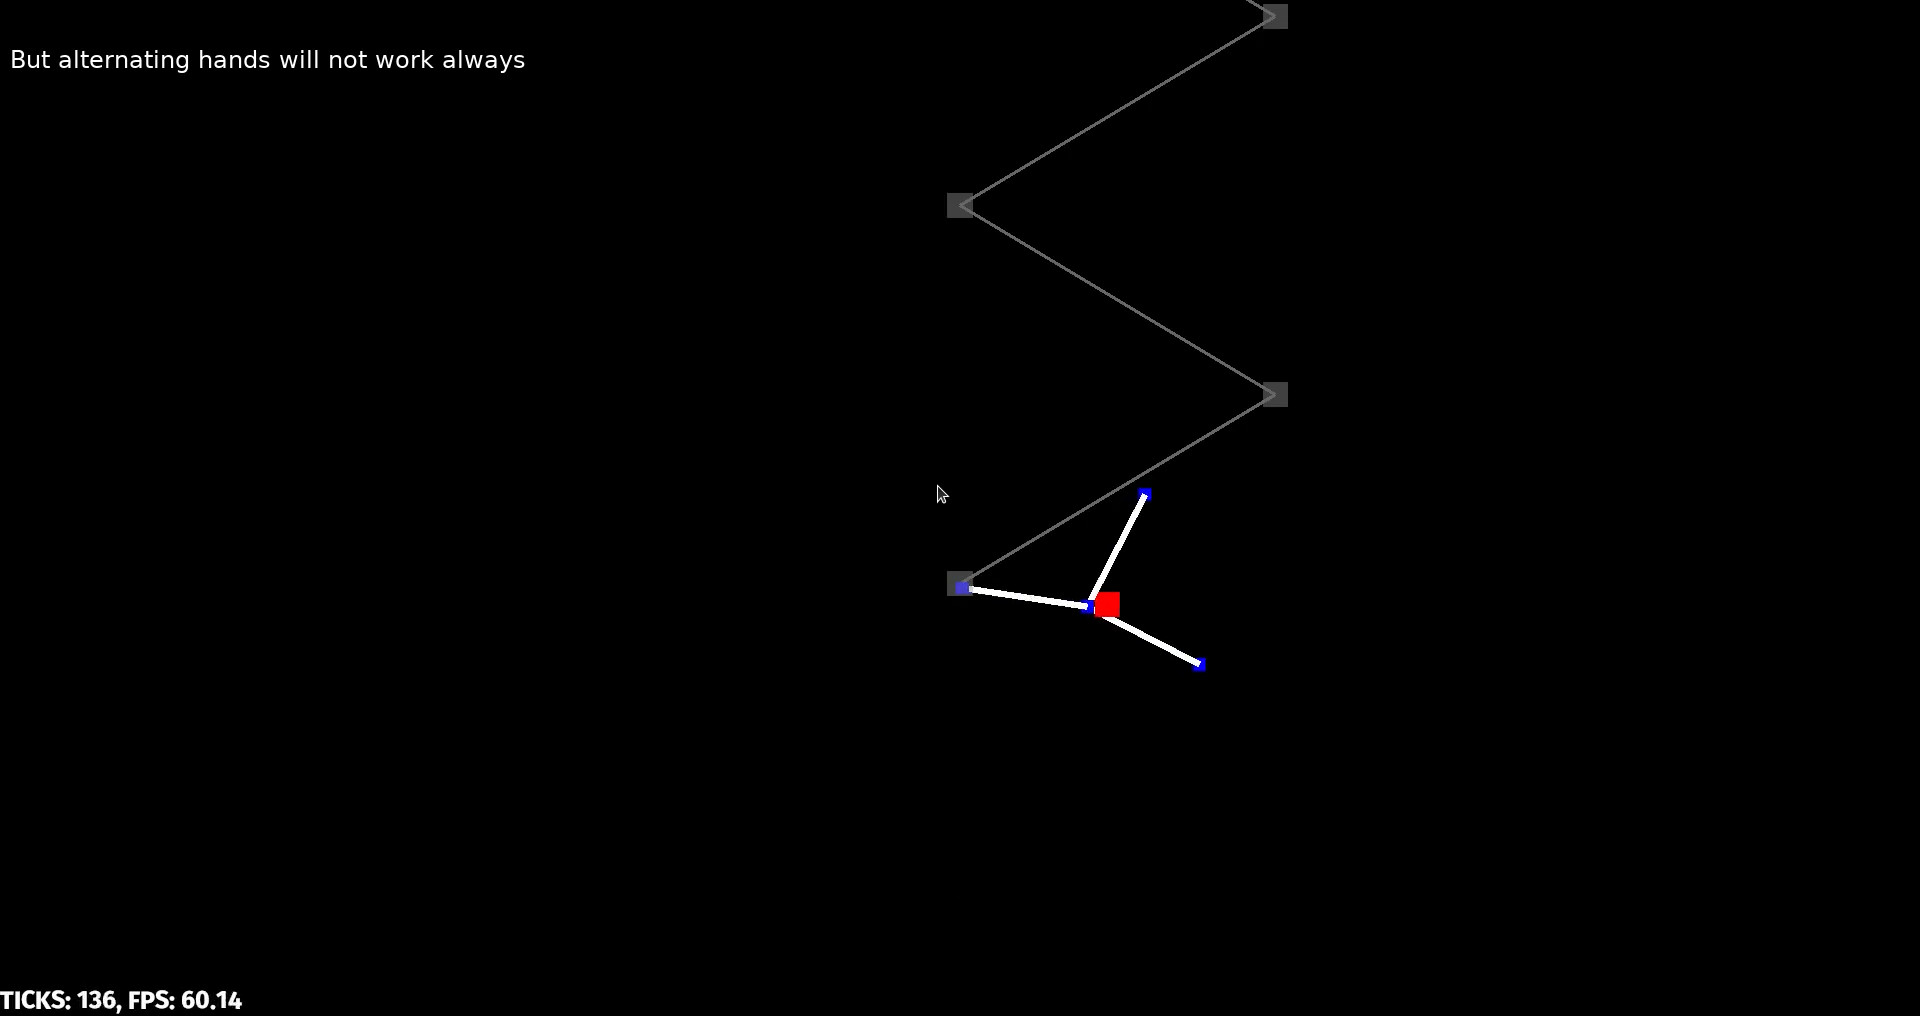
\includegraphics[width=\linewidth]{figures/sf3.jpg}
\endminipage
\caption{Switching pivots for alternating hands results in local minima pose.}
\label{fig:sf}
\end{figure}
\begin{figure}[!htb]
\minipage{0.25\textwidth}
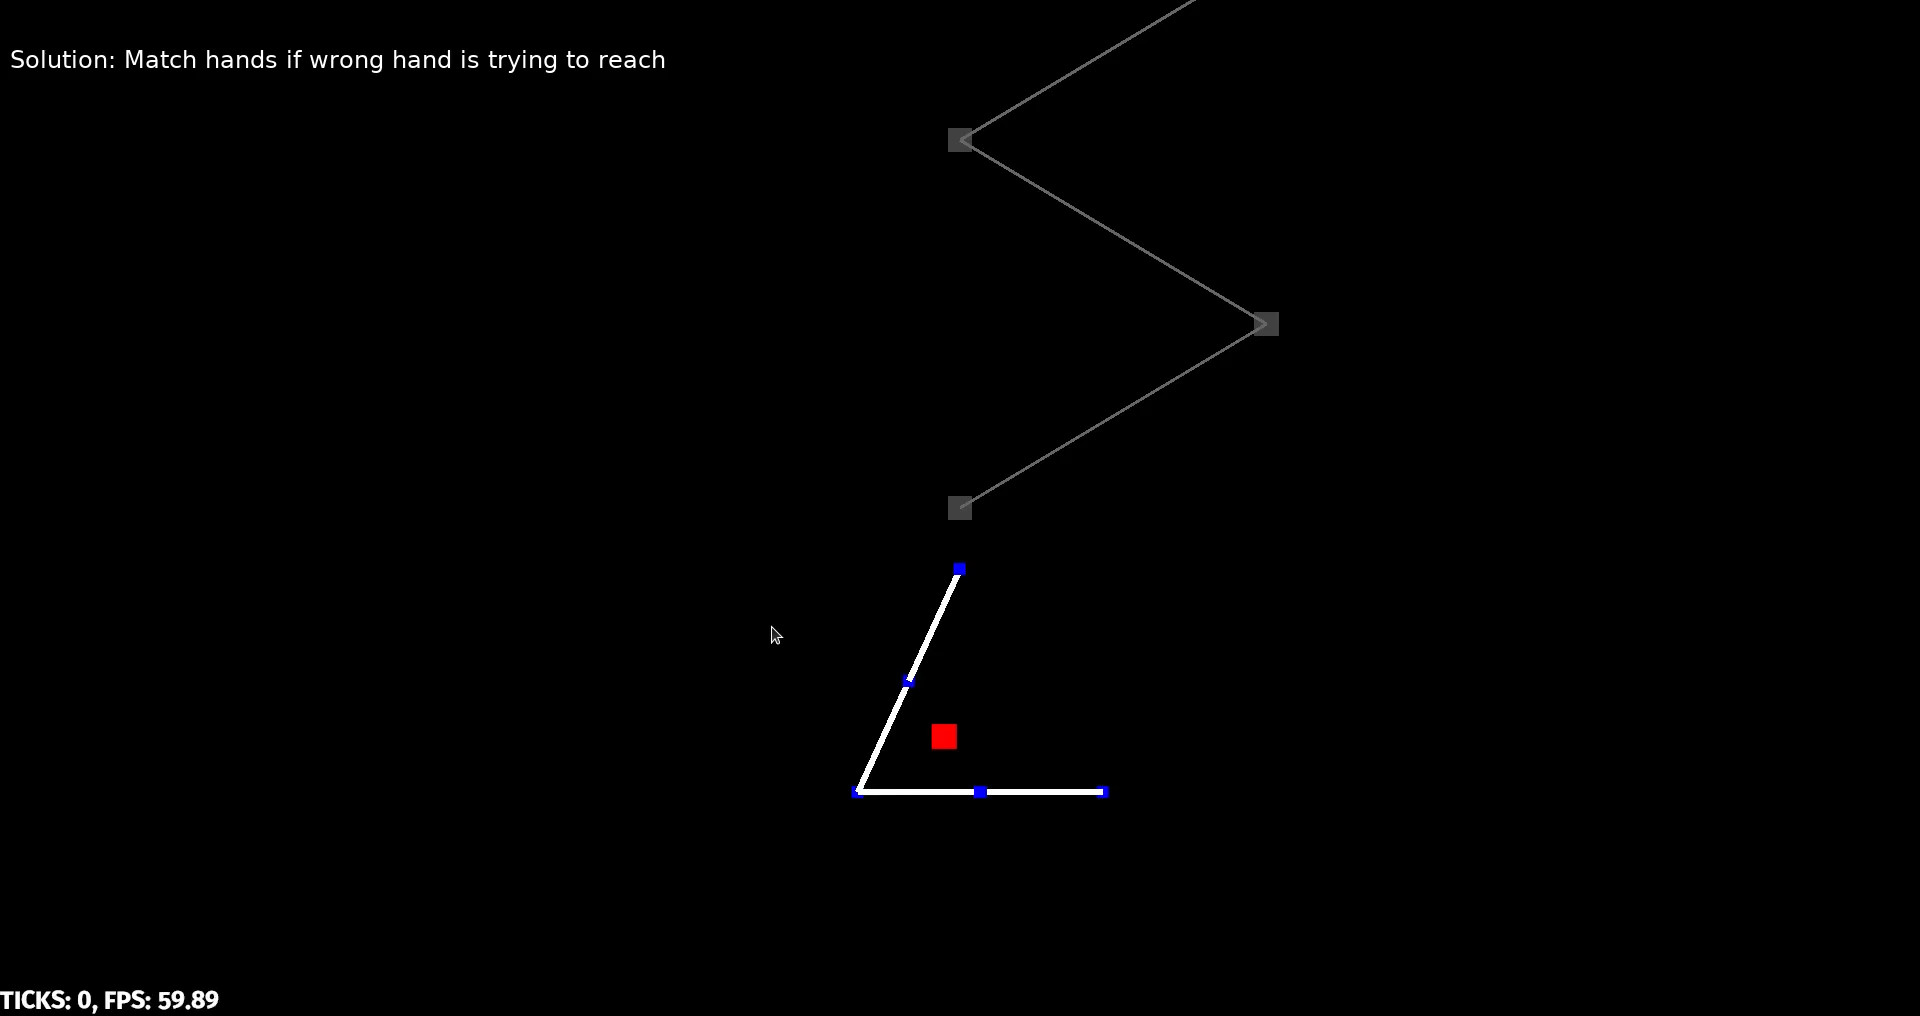
\includegraphics[width=\linewidth]{figures/m1.jpg}
\endminipage\hfill
\minipage{0.25\textwidth}
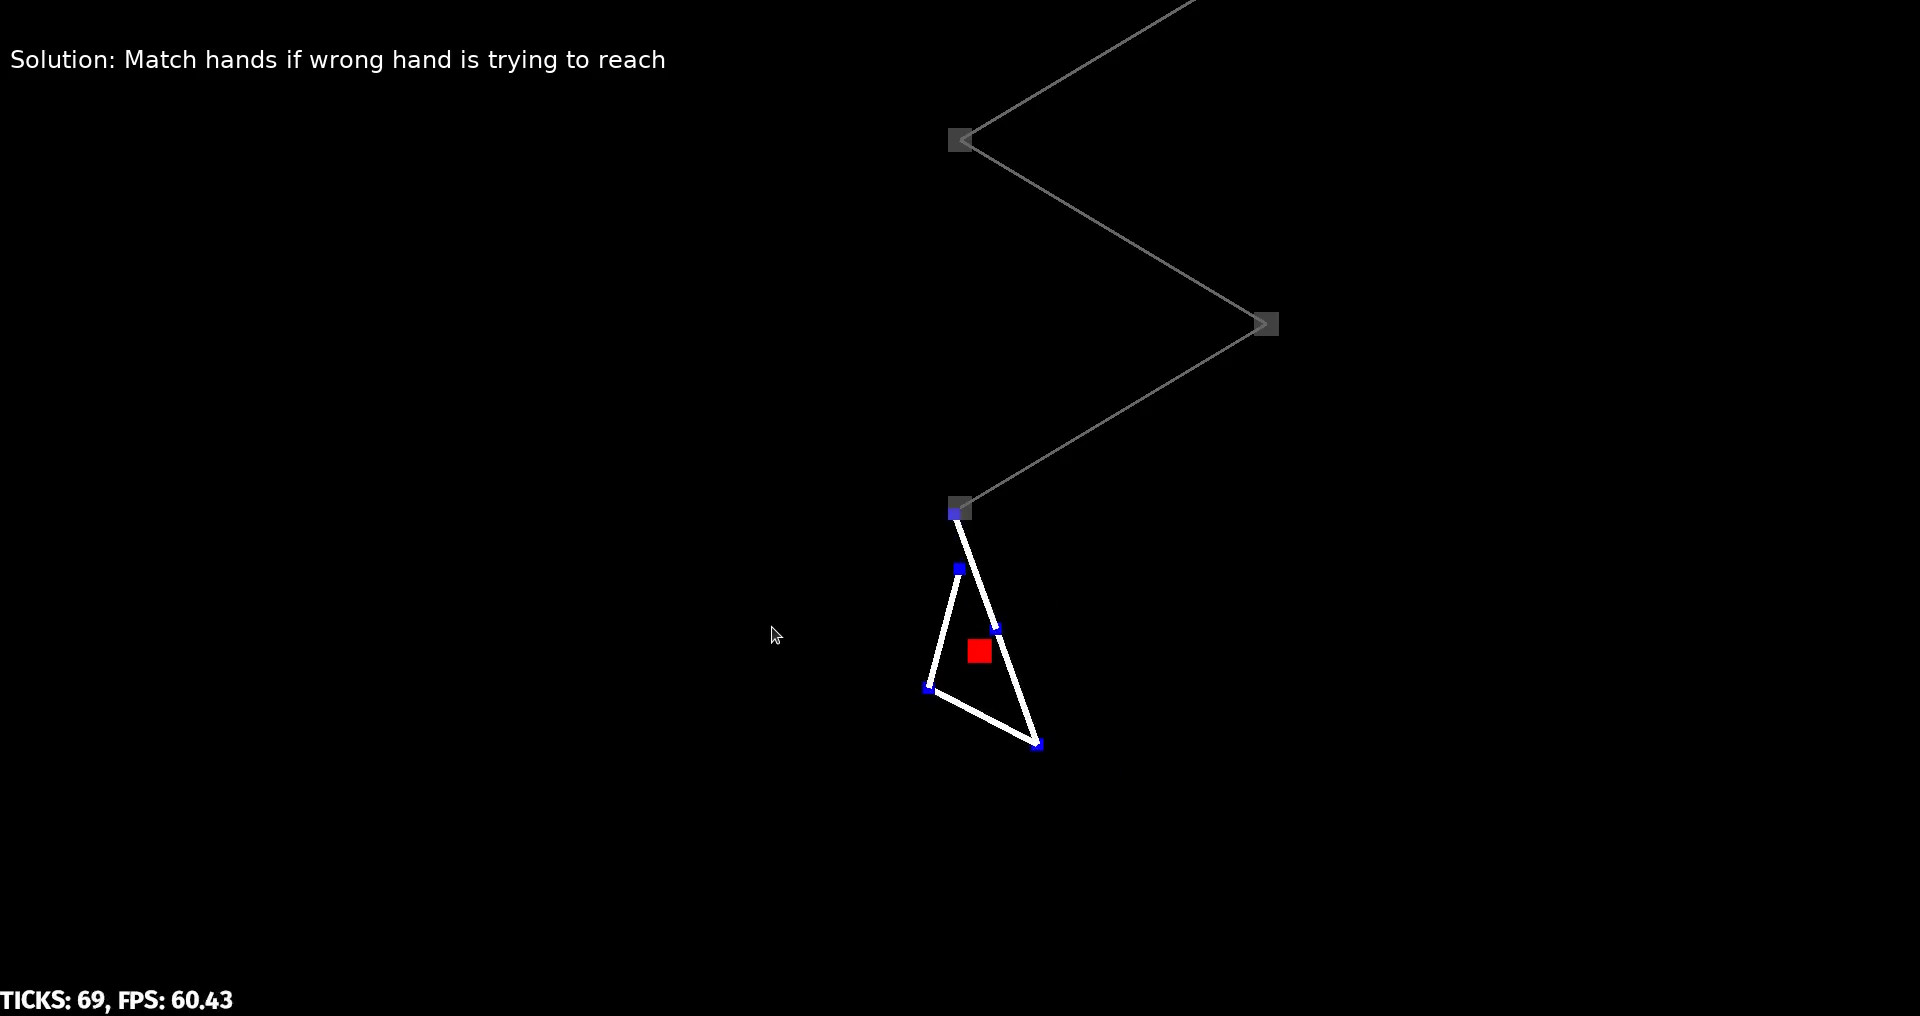
\includegraphics[width=\linewidth]{figures/m2.jpg}
\endminipage\hfill
\minipage{0.25\textwidth}
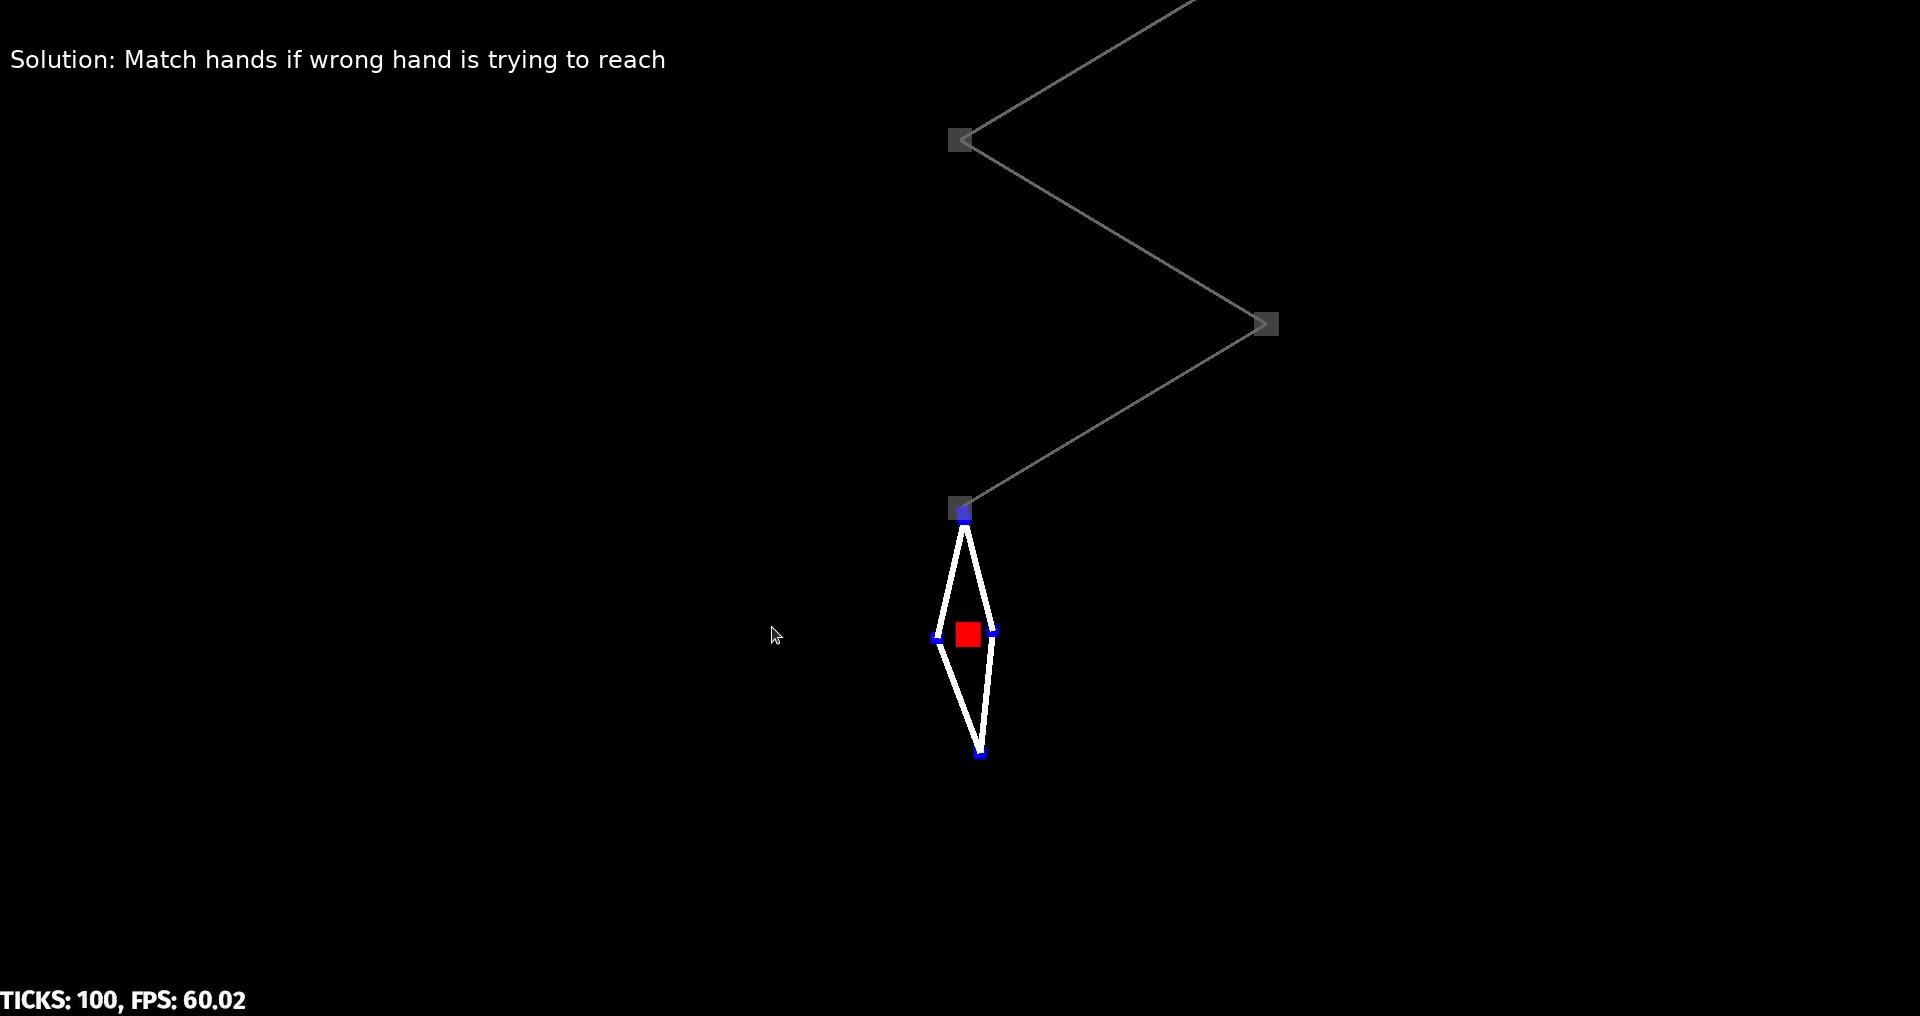
\includegraphics[width=\linewidth]{figures/m3.jpg}
\endminipage\hfill
\minipage{0.25\textwidth}
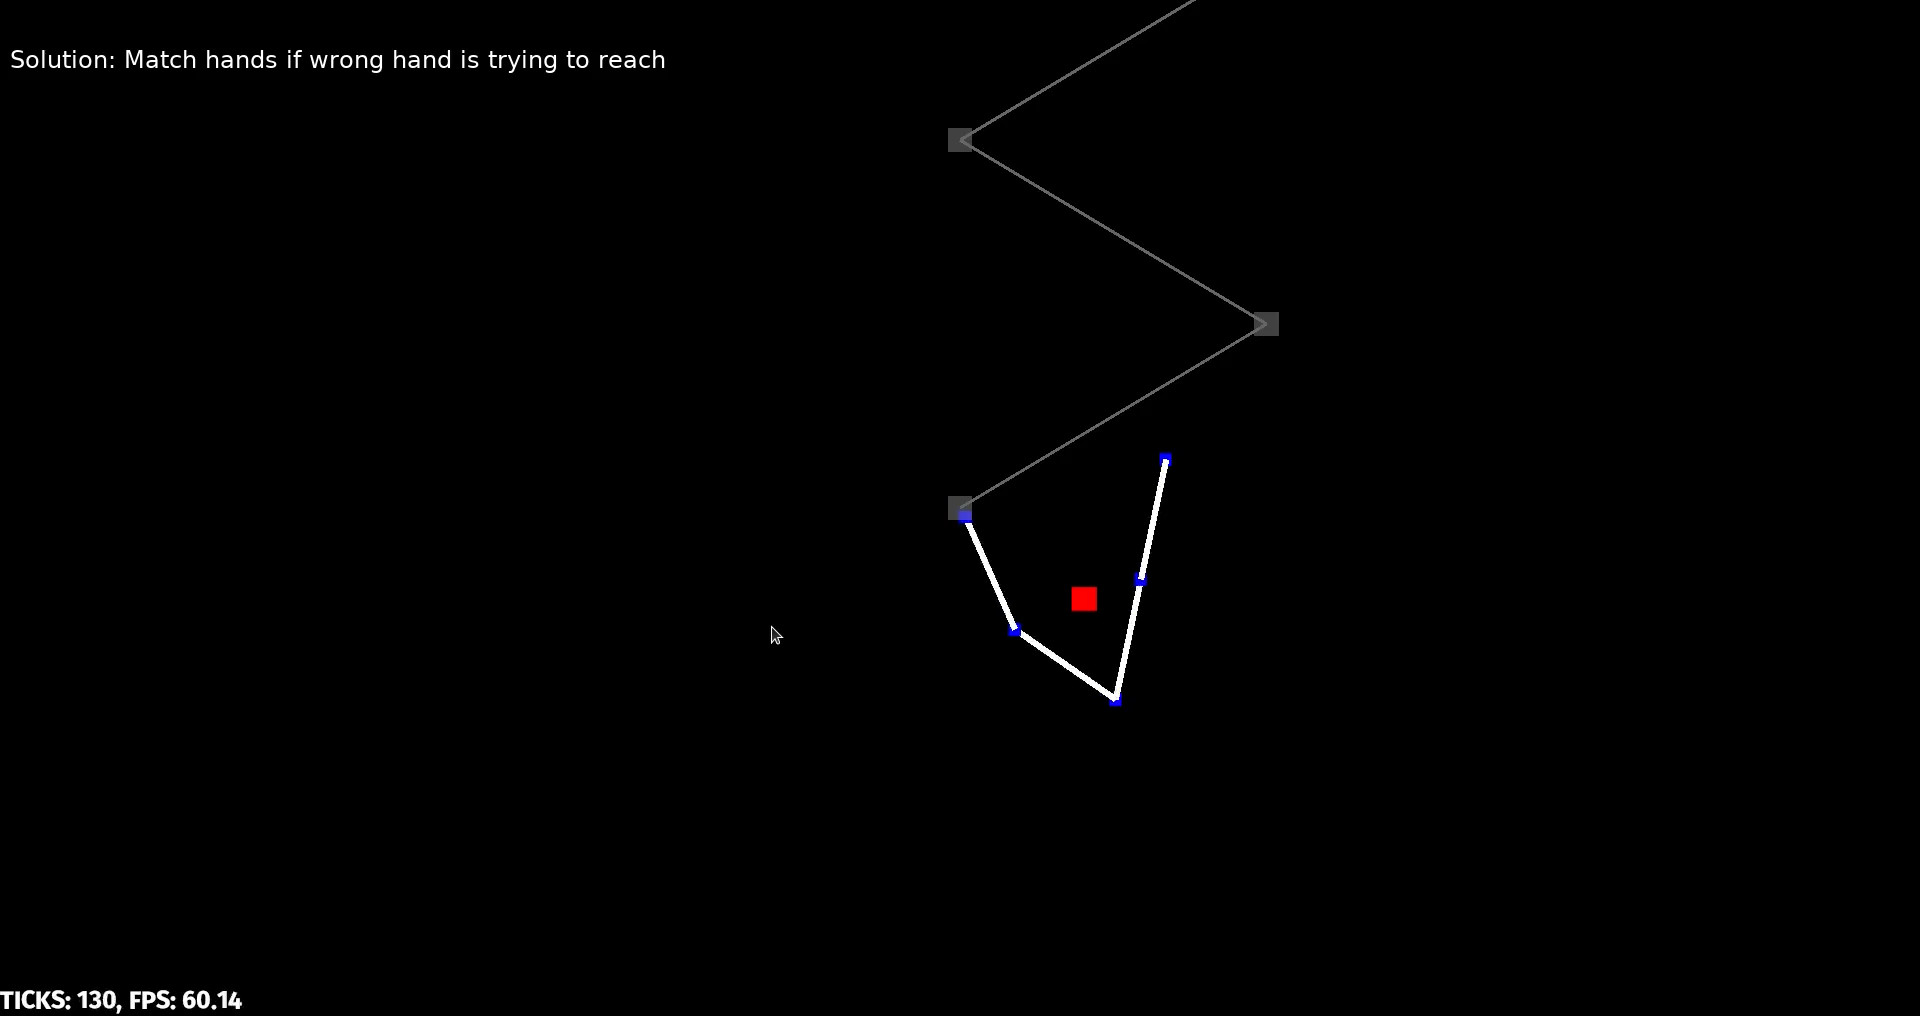
\includegraphics[width=\linewidth]{figures/m4.jpg}
\endminipage\hfill
\caption{Switching pivots + matching hands avoids local minima pose.}
\label{fig:m}
\end{figure}

\subsection{Formulating $2 \times 2R$ limb coordination as an RL problem}
Consider $2 \times 2R$ agent.
We model a pair of arms using this agent.
Since (global + gradient descent) inverse kinematics planners for individual arm (modeled using 2R chain agent) are already in place, we now just plan for the goals of ends of each 2R chain agent.
Again since given a climbing route the goal of non-holding NR chain is determined, the only real variable here is the holding arm goal (i.e. where the neck should go).
Since it is not very trivial as to where the neck should be placed, given a hand goal it is better to use a good function approximator like neural network for this task.
We model this policy as a neural network optimized using cross-entropy method.

\paragraph{Input/Output design}
Since the lower level IK planners take care of current $q$ state, $q$ and $qclamps$ need not be part of input.
It should only depend on current pivot, lengths of links and current goal.
Due to this the policy becomes a discrete control (instead of continuous control) sampled at every pivot switch.
This hugely decreases the burden on the network and really only outsources the most proper work to the network viz. holding arm goal prediction.
This is reflected in the training where good results are achieved in relatively small training times.
Further more, now in order to test the network we just need to check the predictions for goal positions, instead of pair of start and goal positions.
Finally to make the system pivot shift and scale invariant we choose input as a concatenated vector of lengths of holding arm and non-holding arm and goal relative to pivot all of them scaled by sum of all lengths of links.
The output is a two dimensional vector specifying the neck goal.
After a prediction is made we scale back and shift the output before further use.

\paragraph{Reward function design}
The reward function has multiple components.
During episode we have
\begin{enumerate}[nolistsep]
    \item Distance of holding arm end to its goal.
    \item Distance of non-holding arm end to its goal.
    \item Value of com$_y$.
    \item Distance of com$_x$ from its goal.
\end{enumerate}
Since the input is scaled and shifted the rewards can be directly applied without any more pre-processing.
The weights of distance from goal are generally more than those for com.
Since we are using raw value of com$_y$ as a reward, we need to make sure that we sample many goals in the training area for each model, or else some good model can be thrown out for being unfairly tested just on high lying goals.
After the episode we have
\begin{enumerate}[nolistsep]
    \item High reward for distance of holding arm end to its goal being small.
    \item High reward for distance of non-holding arm end to its goal being small.
\end{enumerate}
These rewards ensure the arm reaching the hold.

\paragraph{Network design}
The network used is simple fully connected network with two hidden layers of ReLU activation each with 16 nodes.
Since the problem given to the network is quite simple a small network generally suffices.
We have also tried Sigmoid activations but that did not work as well.

\paragraph{CEO parameters}
Table \ref{tab:ceo} shows cross entropy optimizer parameters used.
It is parallelized on CPU cores and achieves a speedup of 36\% on 8 cores for the parameters given in the table as illustrated in \ref{fig:speedup}.

\begin{table}
\begin{center}
\begin{tabular}{ c c }
key & value \\
\hline
generations & 500 \\
batch\_size & 50 \\
num\_episodes & 20 \\
num\_episode\_ticks & 200 \\
elite\_frac & 0.25 \\
initial\_std & 1.0 \\
noise\_factor & 1.0 \\
\end{tabular}
\end{center}
\caption{Cross entropy optimizer parameters.}
\label{tab:ceo}
\end{table}

\begin{figure}[!htb]
\minipage{0.99\textwidth}
\includegraphics[width=\linewidth]{figures/parallelization.png}
\endminipage\hfill
\caption{Speedup of cross entropy optimization using CPU parallelization.}
\label{fig:speedup}
\end{figure}

\paragraph{Left and right holding networks}
Since the cases where the agent holds the pivot using left hand and right hand can be treated as separate problems, we train two networks, one of each case.
These are called Left and right holding networks.
This further reduces the training time and achieves differing dexterous behavior.

\paragraph{Policy visualization}
Our design of input/output is such that for a given agent (the lengths are fixed) the policy is a mapping from $\mathbb{R}^2 \to \mathbb{R}^2$ (non-holding goal to holding goal).
Because of this low dimensionality the policy can be visualized well.
The figures \ref{fig:lm}, \ref{fig:ld}, \ref{fig:lt} visualize left holding network.
The figures \ref{fig:rm}, \ref{fig:rd}, \ref{fig:rt} visualize right holding network.
These visualizations helped a lot in the design and debugging of reward function, optimizer and the network.
\begin{figure}[!htb]
\minipage{0.49\textwidth}
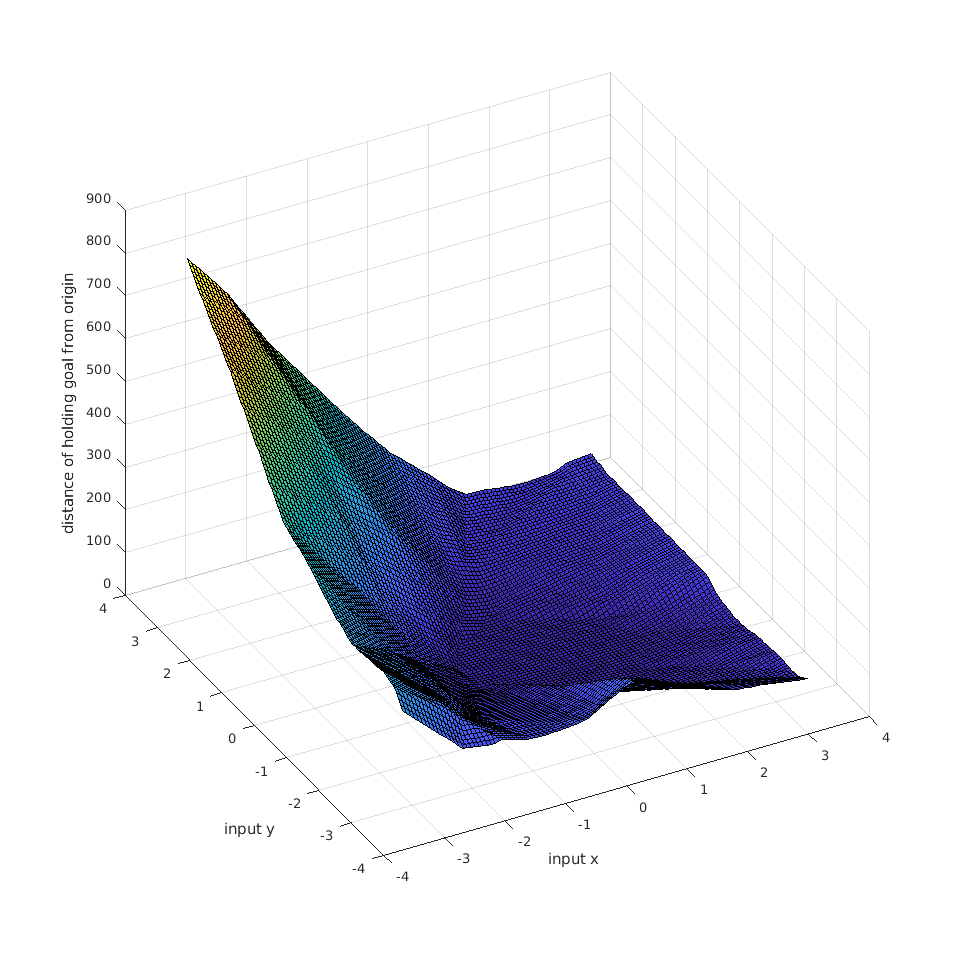
\includegraphics[width=\linewidth]{figures/left/zoomed_out.png}
\endminipage\hfill
\minipage{0.49\textwidth}
\includegraphics[width=\linewidth]{figures/left/zoomed_in.png}
\endminipage\hfill
\caption{For the left holding network, distance of neck goal w.r.t hand goal. Left side shows zoomed out graph, right side shows zoomed in graph. Notice the valley of good predictions among the hills of random noise.}
\label{fig:lm}
\end{figure}
\begin{figure}[!htb]
\minipage{0.99\textwidth}
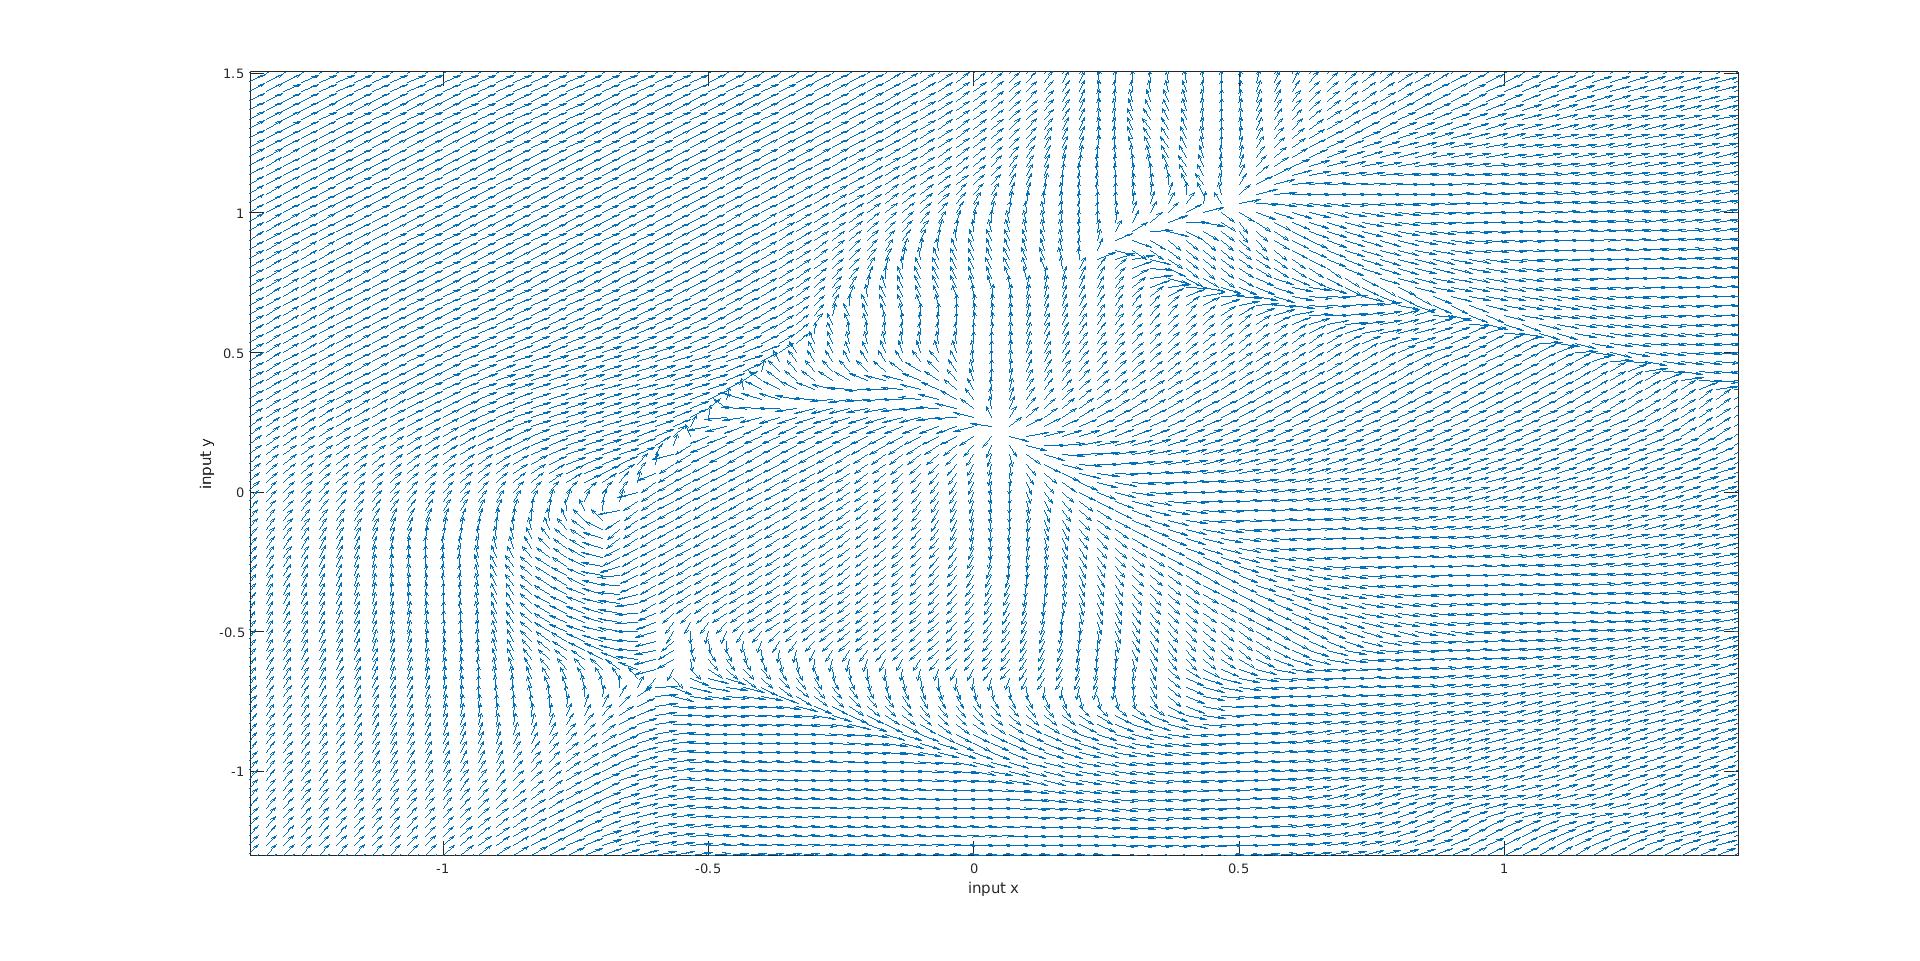
\includegraphics[width=\linewidth]{figures/left/direction.png}
\endminipage\hfill
\caption{For the left holding network, direction of neck goal w.r.t. hand goal.}
\label{fig:ld}
\end{figure}
\begin{figure}[!htb]
\minipage{0.49\textwidth}
\includegraphics[width=\linewidth]{figures/left/original.png}
\endminipage\hfill
\minipage{0.49\textwidth}
\includegraphics[width=\linewidth]{figures/left/mapped.png}
\endminipage\hfill
\caption{For the left holding network, texture distortion map. On the left side is the original texture, on the right is the mapped texture. Notice the smooth predictions in the trained region (right) and noisy predictions in the untrained region (left). Pivot is in the center.}
\label{fig:lt}
\end{figure}

\begin{figure}[!htb]
\minipage{0.49\textwidth}
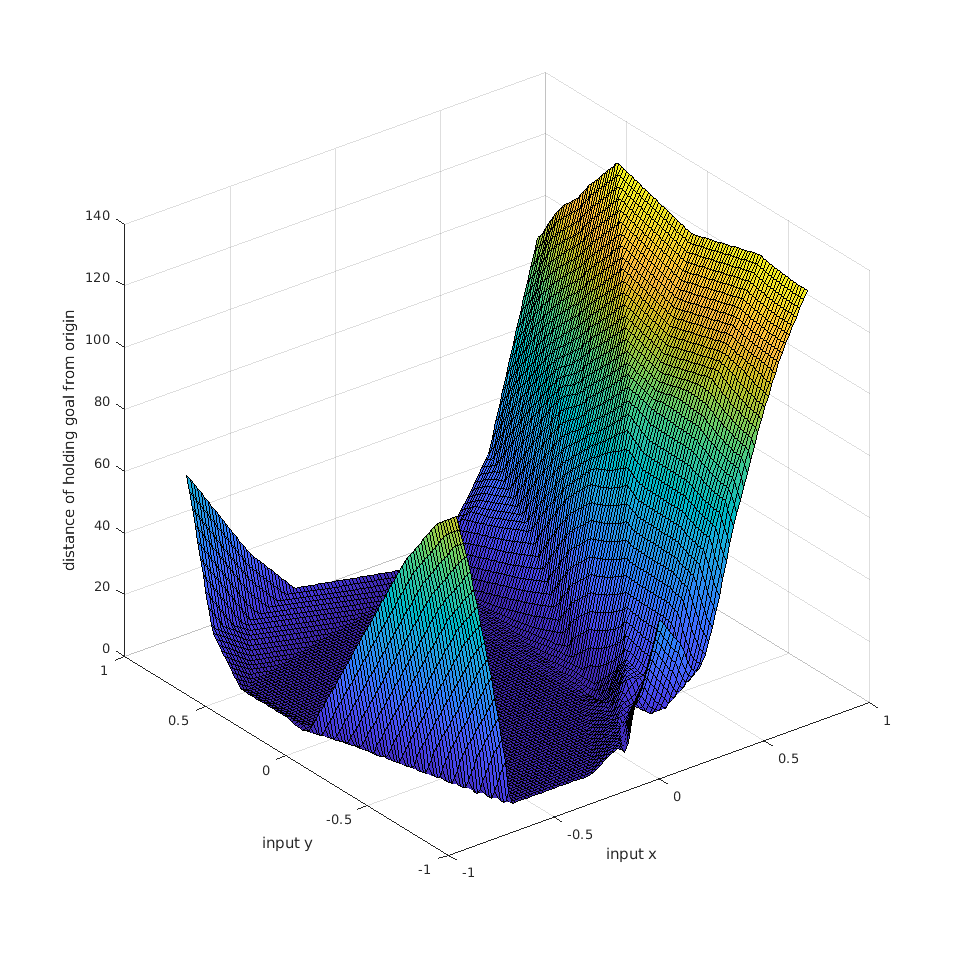
\includegraphics[width=\linewidth]{figures/right/zoomed_out.png}
\endminipage\hfill
\minipage{0.49\textwidth}
\includegraphics[width=\linewidth]{figures/right/zoomed_in.png}
\endminipage\hfill
\caption{For the right holding network, distance of neck goal w.r.t hand goal. Left side shows zoomed out graph, right side shows zoomed in graph. Notice the valley of good predictions among the hills of random noise.}
\label{fig:rm}
\end{figure}
\begin{figure}[!htb]
\minipage{0.99\textwidth}
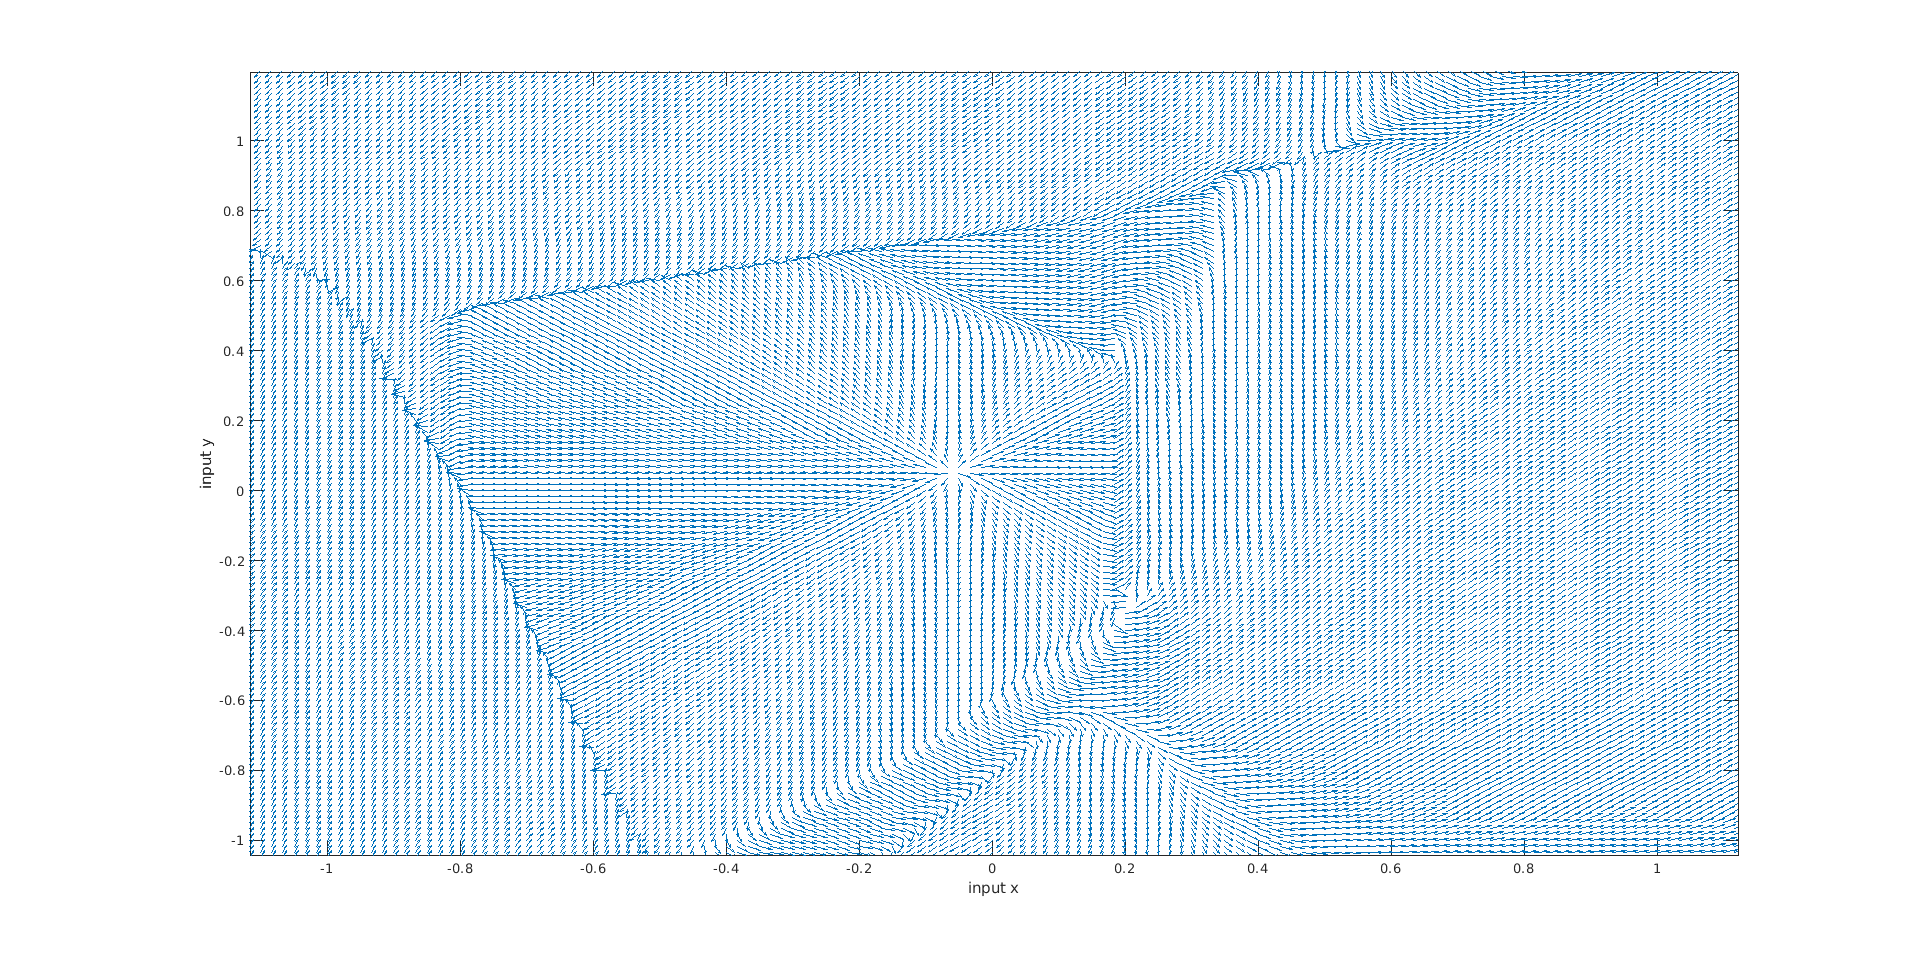
\includegraphics[width=\linewidth]{figures/right/direction.png}
\endminipage\hfill
\caption{For the right holding network, direction of neck goal w.r.t. hand goal.}
\label{fig:rd}
\end{figure}
\begin{figure}[!htb]
\minipage{0.49\textwidth}
\includegraphics[width=\linewidth]{figures/right/original.png}
\endminipage\hfill
\minipage{0.49\textwidth}
\includegraphics[width=\linewidth]{figures/right/mapped.png}
\endminipage\hfill
\caption{For the right holding network, texture distortion map. On the left side is the original texture, on the right is the mapped texture. Notice the smooth predictions in the trained region (left) and noisy predictions in the untrained region (right). Pivot is in the center.}
\label{fig:rt}
\end{figure}

\section{experiments and results}
We first model two arms using a 4R agent controlled by
\begin{enumerate}[nolistsep]
    \item Vanilla gradient descent.
    \item Gradient descent + relaxation on every hold.
    \item No prior random sampling solve + gradient descent.
    \item Current state random sampling solve + gradient descent.
\end{enumerate}
All of these are tested on the same sophisticated climbing route involving left/right, up/down and diagonal moves.
The standard route is shown in figure \ref{fig:route}.

\begin{figure}[!htb]
\minipage{0.99\textwidth}
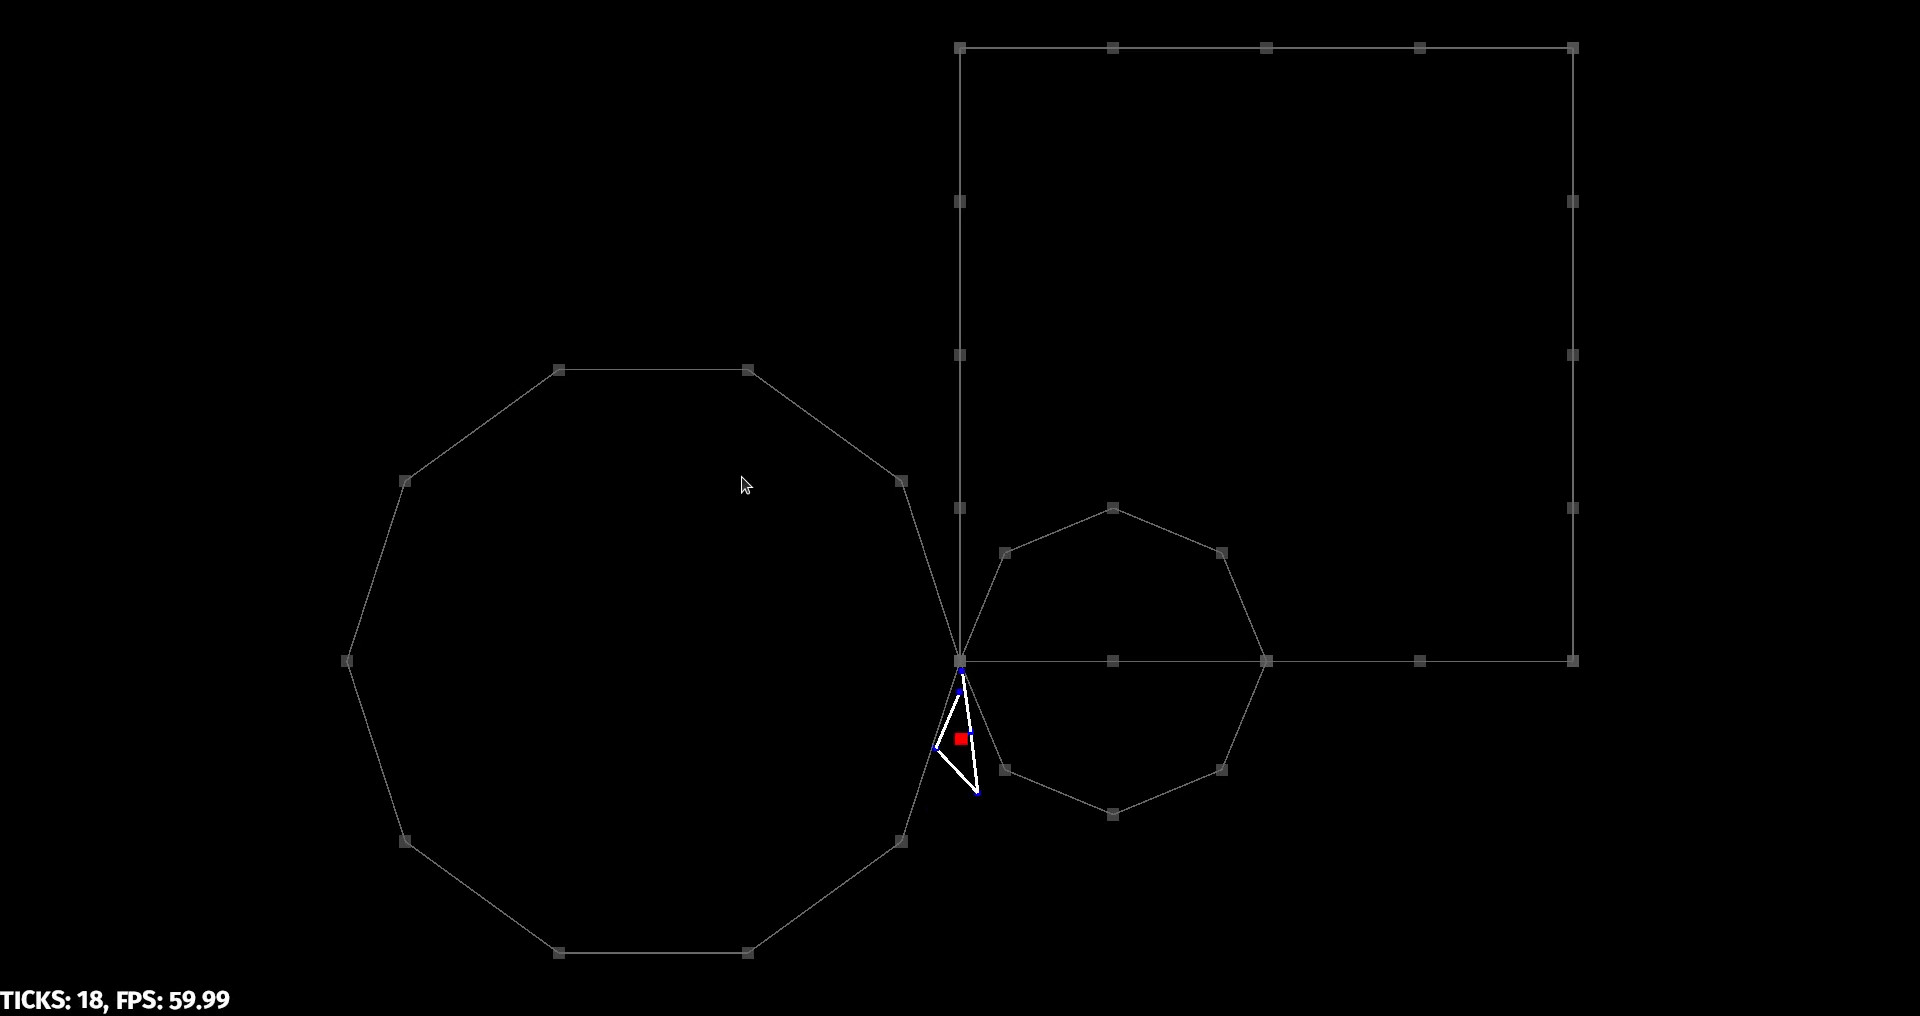
\includegraphics[width=\linewidth]{figures/route.jpg}
\endminipage\hfill
\caption{Standard climbing route: grey points represent holds, edges represent path. Route: left circle counter clockwise, right circle clockwise and then square in clockwise.}
\label{fig:route}
\end{figure}

\begin{enumerate}[nolistsep]
    \item Vanilla gradient descent is simple but quickly gets stuck in local minima pose and cannot proceed.
    \item Gradient descent + relaxation on every hold performs a little better but tuning the relaxation time is difficult and agent still generally gets stuck. Also using this method the agent reaches goal terribly slowly due to all the relaxation.
    \item No prior random sampling solve + gradient descent does not get stuck in local minima, is decently fast and makes the agent reach the final hold pretty consistently.
    \item Current state random sampling solve + gradient descent is also decently fast and makes the agent reach the final hold pretty consistently. For this method the vicinity region parameter has to be tuned to avoid local minima poses.
\end{enumerate}
\\\\
We then model two arms using a $2 \time 2R$ agent controlled by cross-entropy optimized network.
It is also tested on the same climbing route.
This agent is also quite fast and finishes the route pretty consistently.
This demonstrates the aspect of multi-limb coordination.
Please refer to supplementary video for demonstration.
\\\\
All the random global solves use randomness at their core and therefore produce different motion for same condition on each run.
\paragraph{Comparison to baseline}
\begin{enumerate}[nolistsep]
    \item Baseline has no constraints on $q_i$ and $\Delta q_i$. The current version has them.
    \item Baseline has no explicit center of mass considerations. The current version has tunable center of mass control.
    \item Baseline has no multi-limb coordination. The current version uses RL for that.
    \item Baseline mainly uses gradient descent on loss function. The current version mainly uses globally optimal solves with gradient descent just for snapping on to a hold once close enough, thus avoiding local minina poses.
\end{enumerate}

\section{conclusion}
We started out with the goal
\begin{enumerate}[nolistsep]
    \item To model human-like motion using simple heuristics.
    \item To generate a controller for a given agent so that it reaches the finish hold.
\end{enumerate}
Using the simple center of mass control we were able to make the motion significantly more natural looking.
The near globally optimal random sample solves + gradient descent provides good planning stack for inverse kinematics level by avoiding local minima poses and preferring joint angles or enforcing joint angle constraints. The cross-entropy optimized neural network makes a good higher level planner which guides the lower level IK planner.

\paragraph{Biases}
There are no datasets involved in this work.
No simulator was used for this work hence any heuristics used are entirely based on our judgment.
There heuristics may fail completely (although unlikely) in a simulator or real world.
Moreover energy of the agent is limited either as a robot or a human, but this is not modeled in this work.

\paragraph{Limitations}
Modeling human motion is done only using the center of mass control.
Tuning for this is a cumbersome and difficult process and still does not guarantee avoiding weird poses.
To resolve this a good physical simulator can be used on which these algorithms can be developed further.
Even after globally optimal solves there is no guarantee that agent reaches the hold in a given amount of time since gradients vanish near local minima.
This was the case with some runs of the best models.
This is a problem for time critical missions.
To resolve this problem one could scale gradients in a better task specific way.
Since this work did not use a simulator, there might also be additional challenges in controlling an agent in a simulator or a real world, like torque limits, precision of motors, friction, air drag, noise etc.

\paragraph{Future work}
Although the methods in this work are shown for a $2 \times 2R$ agent, they can be easily extrapolated to any Tree of NR chains agent, which includes a full human-lik stick figure agent.
The current work does not deal with multiple simultaneous pivots which are essential in actual climbing, where climbers generally uses two holds to hang.
These problems would be a good follow-up work.

\bibliographystyle{apalike}
\bibliography{cites}

\end{document}
